
\addtocounter{part}{3}

\part{Interstellar dust}
%\part[III]{Nebular Astrophysics}
\begin{frame}
  \partpage
  \tableofcontents[part=4]
\end{frame}

\section{Extinction}

\begin{frame}\frametitle{Extinction}


References: 

Draine, B.T., 2003, ``Astrophysics of Dust in Cold Clouds'',
astro-ph/0304488
Draine, B.T., 2004, ARA\&A, 41, 241


\begin{itemize}

\item $A_\lambda \equiv -2.5 \log_{10} I_\mathrm{obs} /
I_\mathrm{int}$. 

\item $I_\mathrm{obs} = \exp(-\tau)  I_\mathrm{int}$
${\bf \Longrightarrow}$ $A_\lambda = 2.5 \tau / \ln(10) \approx 1.086
\tau(\lambda)$. 

\item $A_\lambda$ is measured by comparing magnitudes  for star with
the same spectral type, or else using recombination lines. 





\item $R_V = A_V / E(B-V)   = A_V / (B-V|_\mathrm{obs} - B-V|_\mathrm{int}) = A_V / (A_B - A_V)$

\end{itemize}

\end{frame}
\begin{frame}\frametitle{Extinction}

\begin{itemize}


\item grains $\ll \lambda$: Rayleigh-scattering gives $A_\lambda \propto
\lambda^{-4}$, $R_V \approx 1.2$. 

\item grains $\gg \lambda$: gray extinction, independent of 
$\lambda$, $R_V \rightarrow \infty$.


\item Parametrisation in terms of single parameter  $R_V$ OK for
$\lambda > 3030~$\AA:
\[ A(\lambda),R_V) = a(\lambda)  + b(\lambda) / R_V, \]
where $a(\lambda)$ and $a(\lambda)$ are power laws, set by fitting the
data (Cardelli et al., 1989, ApJ, 345, 245). 

\item For $\lambda < 3030~$\AA~, use $A_\lambda \approx f(\lambda;
R_V,\{a_i\})$ where $\{a_i\}$ charasterise the UV `bump'.

\item In the  IR, between  $0.9$ and  $6\mu\mathrm{m}$, $A_\lambda$ is $\pm$
universal: $A_\lambda = 2.4~\lambda^{-1.75}$ (Draine 1989, quoting
`Infrared Astronomy', Tokunaga in {\em Astrophysical Quantities}).

\end{itemize}


\end{frame}
\begin{frame}\frametitle{Extinction}


\begin{center}
\rotatebox{-90}{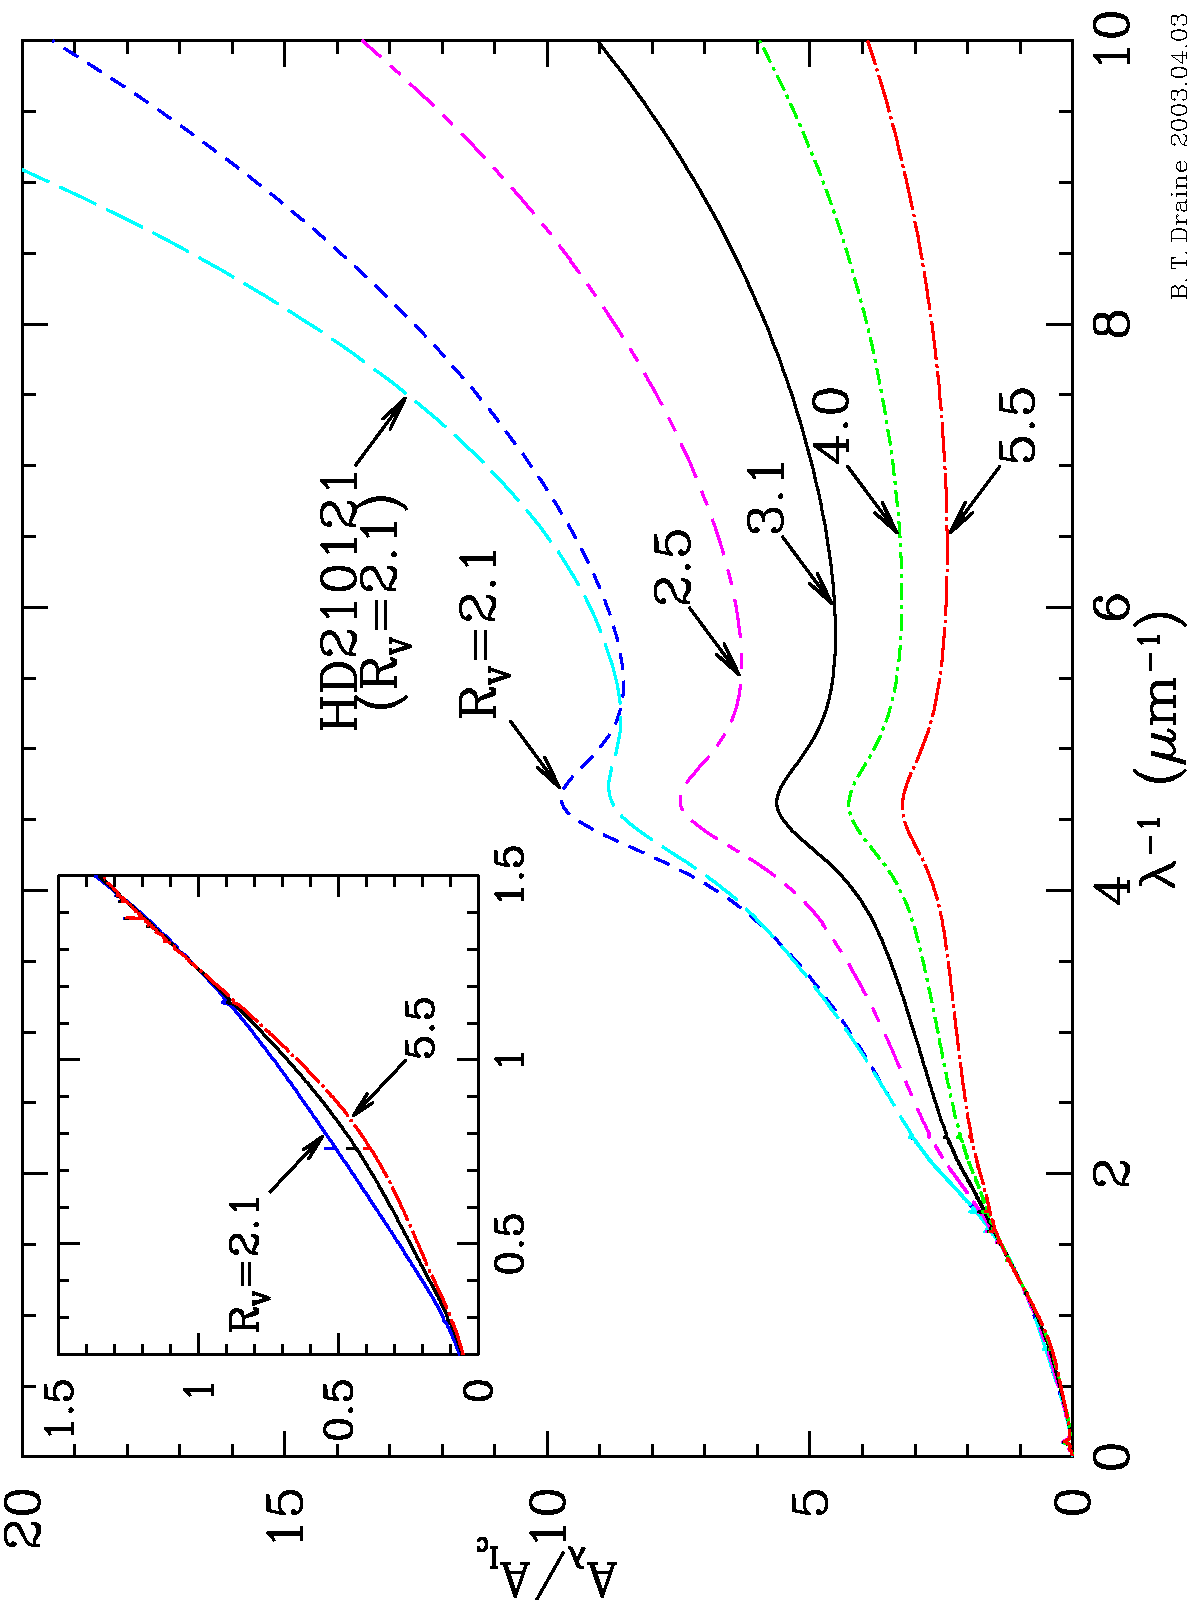
\includegraphics[width=!,height=\textwidth]{./D/draine_araa_f1.pdf}}
\end{center}


\end{frame}
\begin{frame}\frametitle{Extinction}

\begin{center}
\rotatebox{-90}{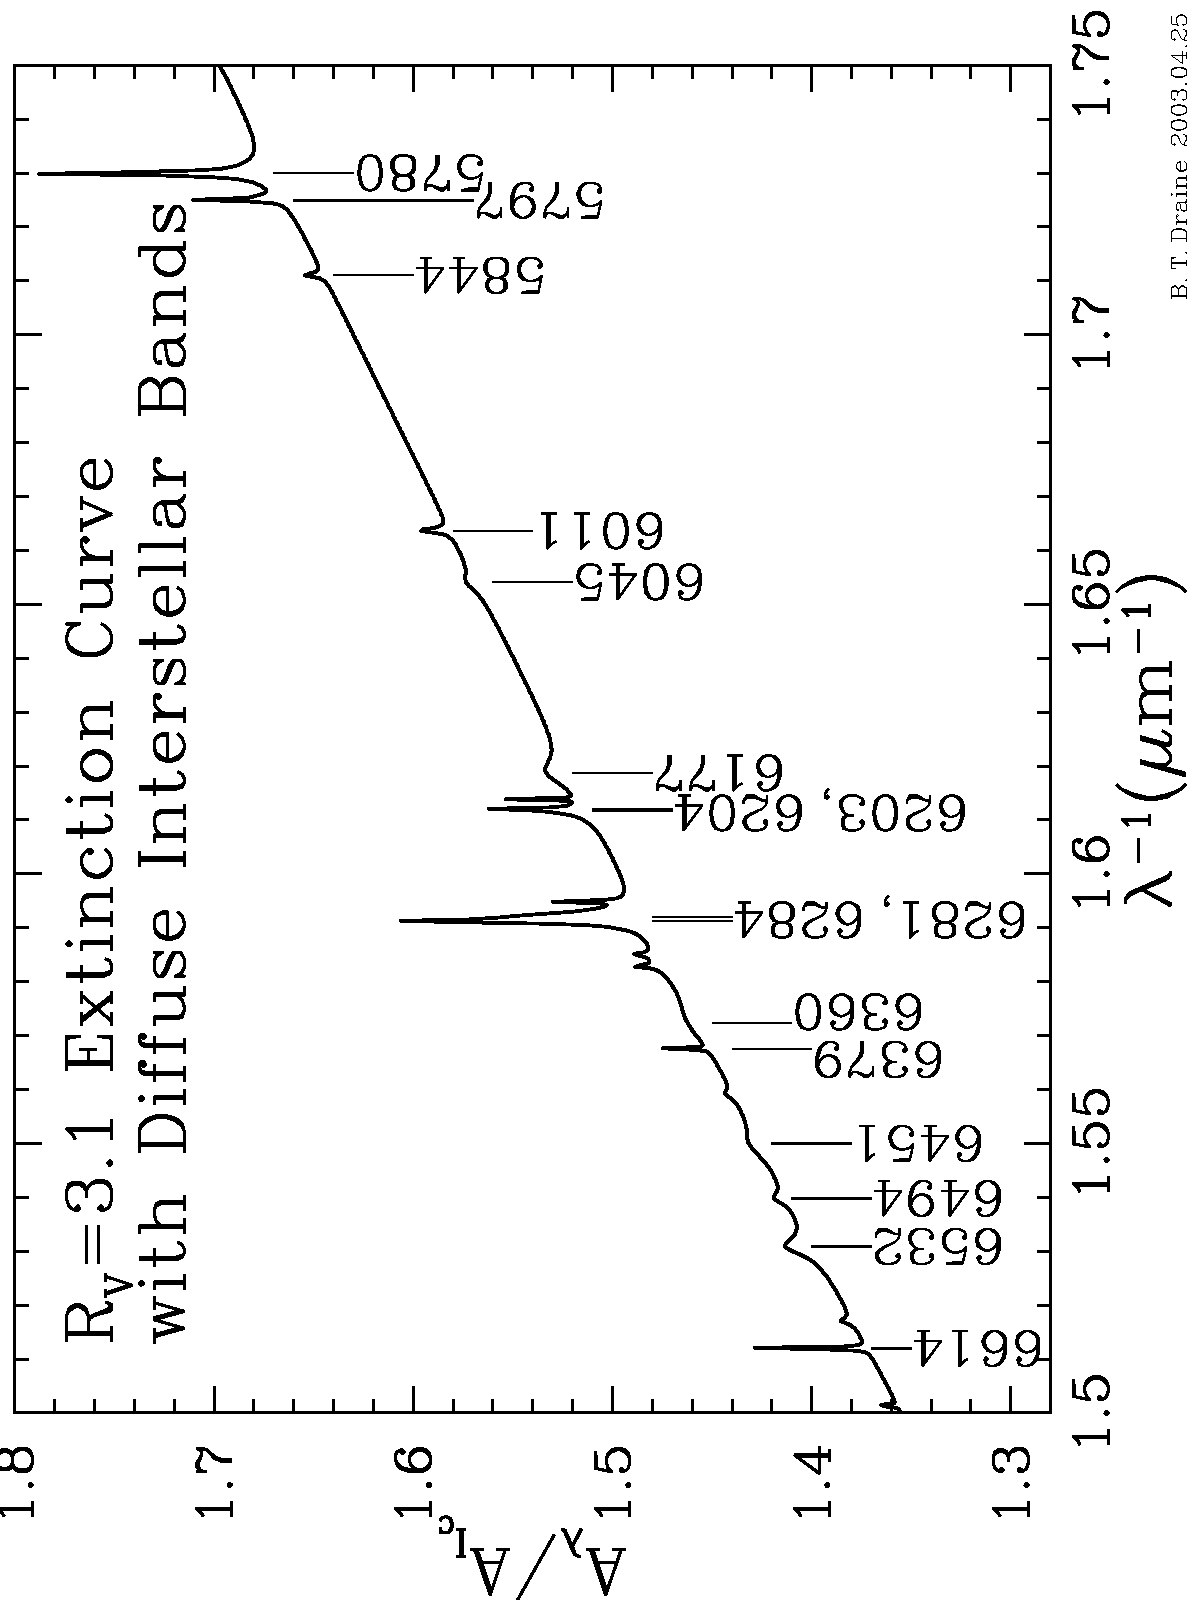
\includegraphics[width=!,height=\textwidth]{./D/draine_araa_f5.pdf}}
\end{center}


\end{frame}
\begin{frame}\frametitle{$R_V$?}



\begin{itemize}
\item Galactic bulge: $R_V = 1.8-2.5$ (Udalski 2002)
\item LMC: $R_V=3.1 $ (Udalski 2002)
\item Cirrus clouds (far from the galactic plane):  $R_V=2 $ (Guhathakurta
1999).
\item Typical value for the local  {\sc ism} : $R_V = 3.1\pm 2$!?
(Cardelli et al 1989)
\end{itemize}


\end{frame}
\begin{frame}\frametitle{$N_H \leftrightarrow A_{V}$\footnote{
ojo: $A_V$ vs $1/R_V \propto 1/A_V$}}


Using H\,{\sc i} Ly$\alpha$ and H$_2$ absorption lines to measure the
column of protons to nearby stars gives $N_H / E(B-V) = 5.8~10^{21}$
cm$^{-2}$mag$^{-1}$, or $N_H / A_V = 1.87~10^{21}$
cm$^{-2}$mag$^{-1}$, for $R_V = 3.1$. But $N_H
\leftrightarrow A_{V}$  varies with sighlines:
\begin{center}
\rotatebox{-90}{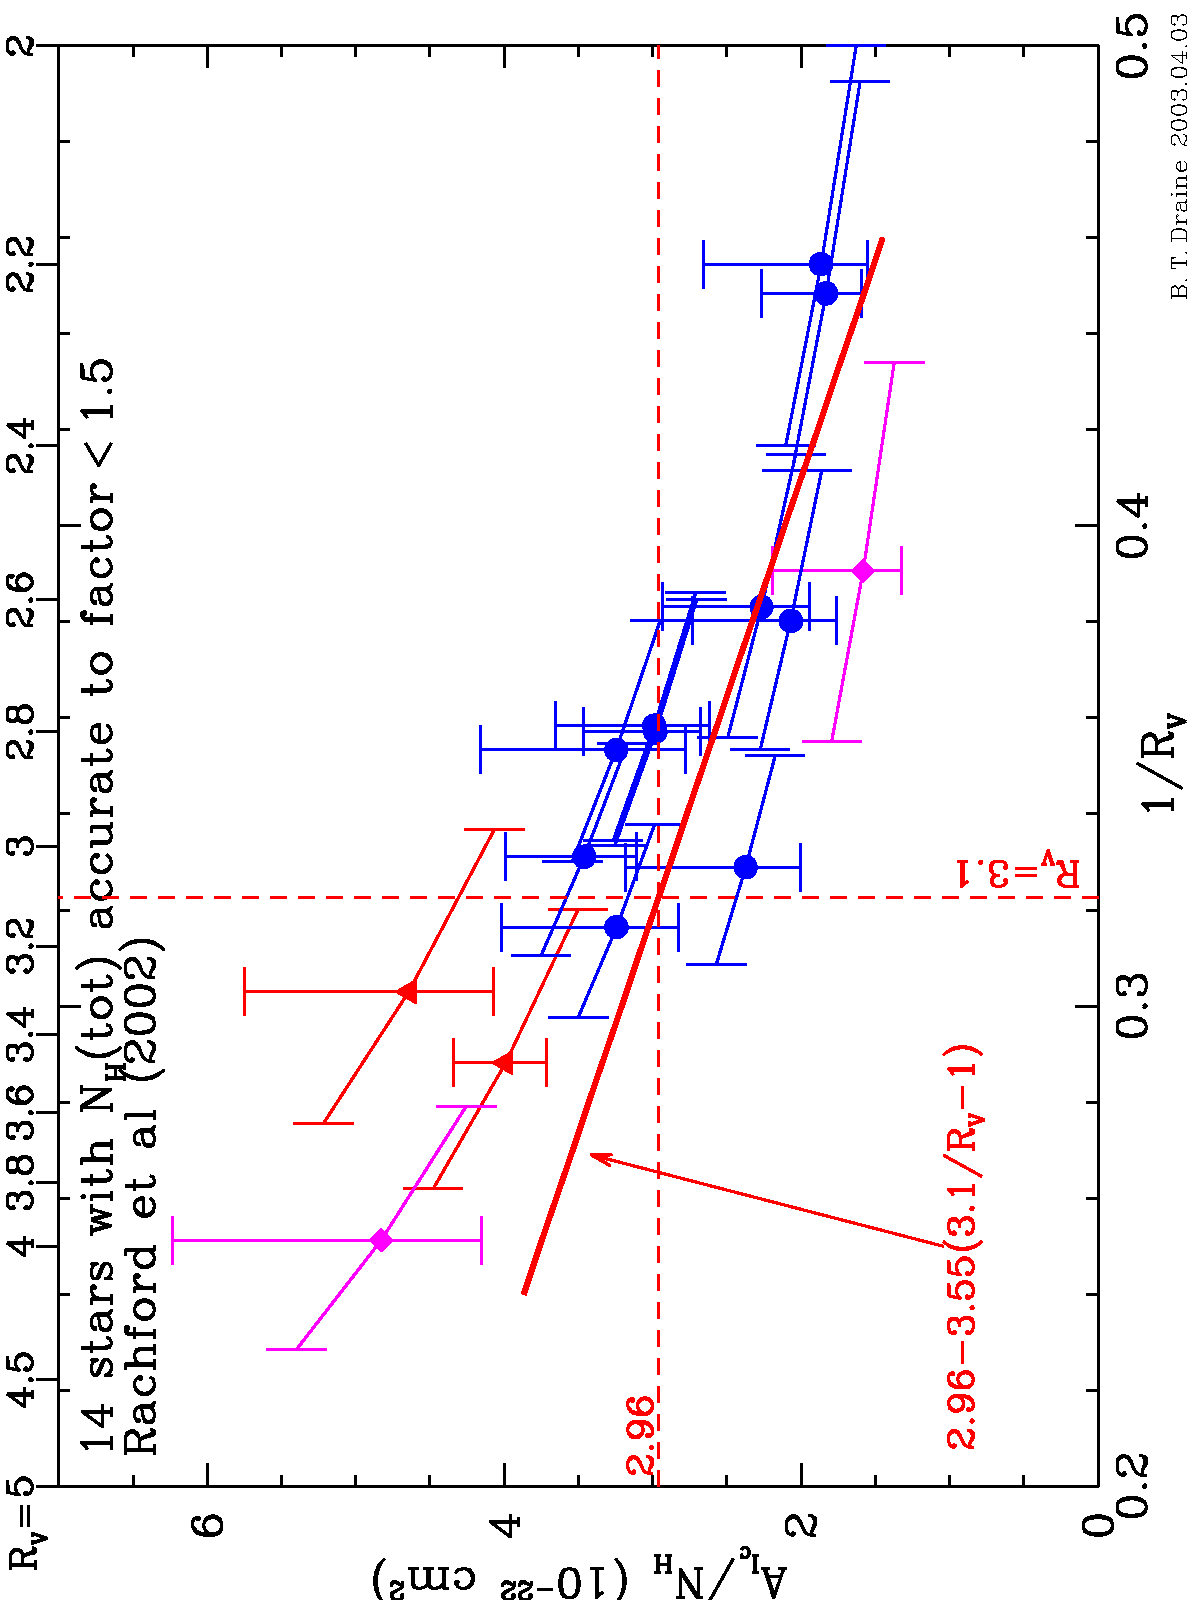
\includegraphics[width=!,height=0.6\textwidth]{./D/draine_araa_f2.pdf}}
\end{center}
$A_V(N_H)$ follows $Z$ in the Magellanic Clouds: 40\% of Milky Way
extinction in LMC, 10\% in SMC.


\end{frame}
\begin{frame}\frametitle{$A_\lambda$ over 6-8~$\mu\mathrm{m}$ }


%\vspace{-1cm}
\begin{center}
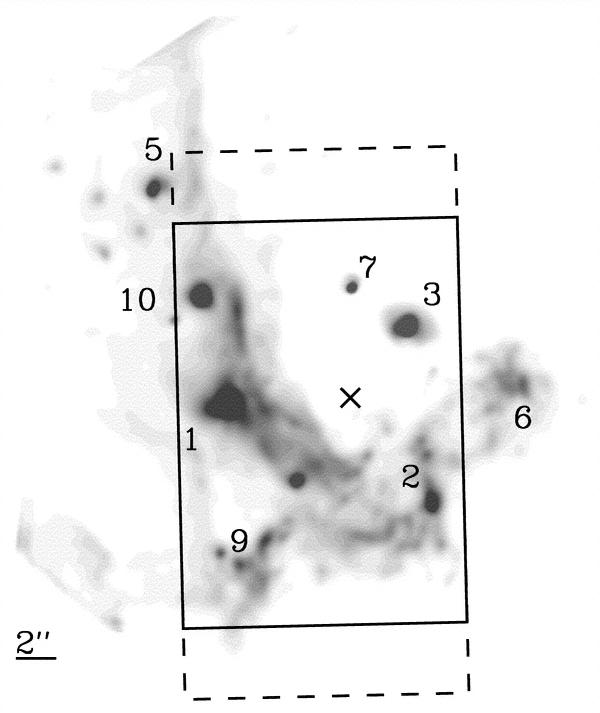
\includegraphics[width=!,height=0.8\textwidth]{./D/ISO_field_GC.jpg}
\end{center}


\end{frame}
\begin{frame}\frametitle{$A_\lambda$ over 6-8~$\mu\mathrm{m}$ }


Lutz et al. (1996, A\&A, 315, L269) find excess extinction assuming
Case B for H recombination lines in the $ISO$+SWS spectrum.
%\vspace{-1cm}
\begin{center}
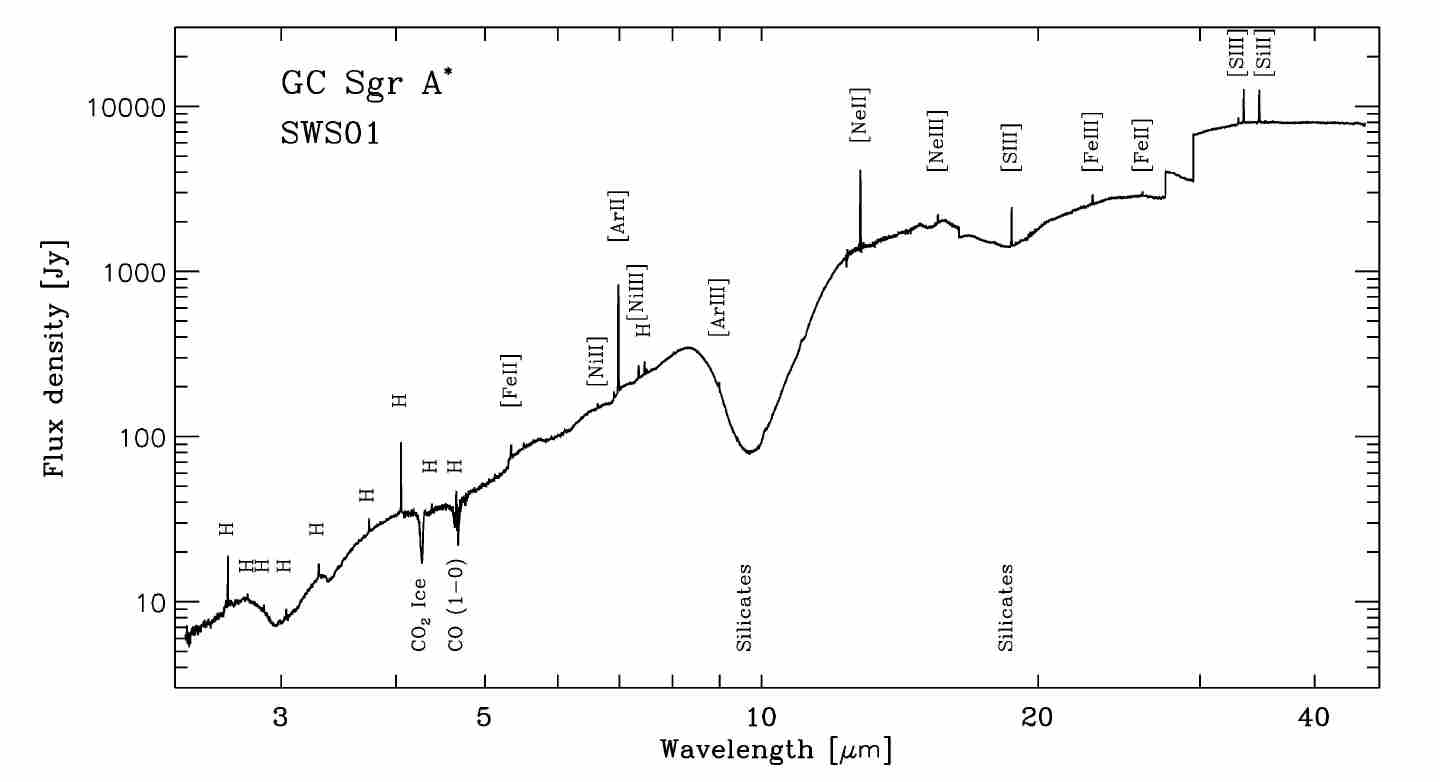
\includegraphics[width=\textwidth,height=!]{./D/iso_GC.jpg}
\end{center}


\end{frame}
\begin{frame}\frametitle{$A_\lambda$ over 6-8~$\mu\mathrm{m}$ }


%\vspace{-1cm}
\begin{center}
\rotatebox{-90}{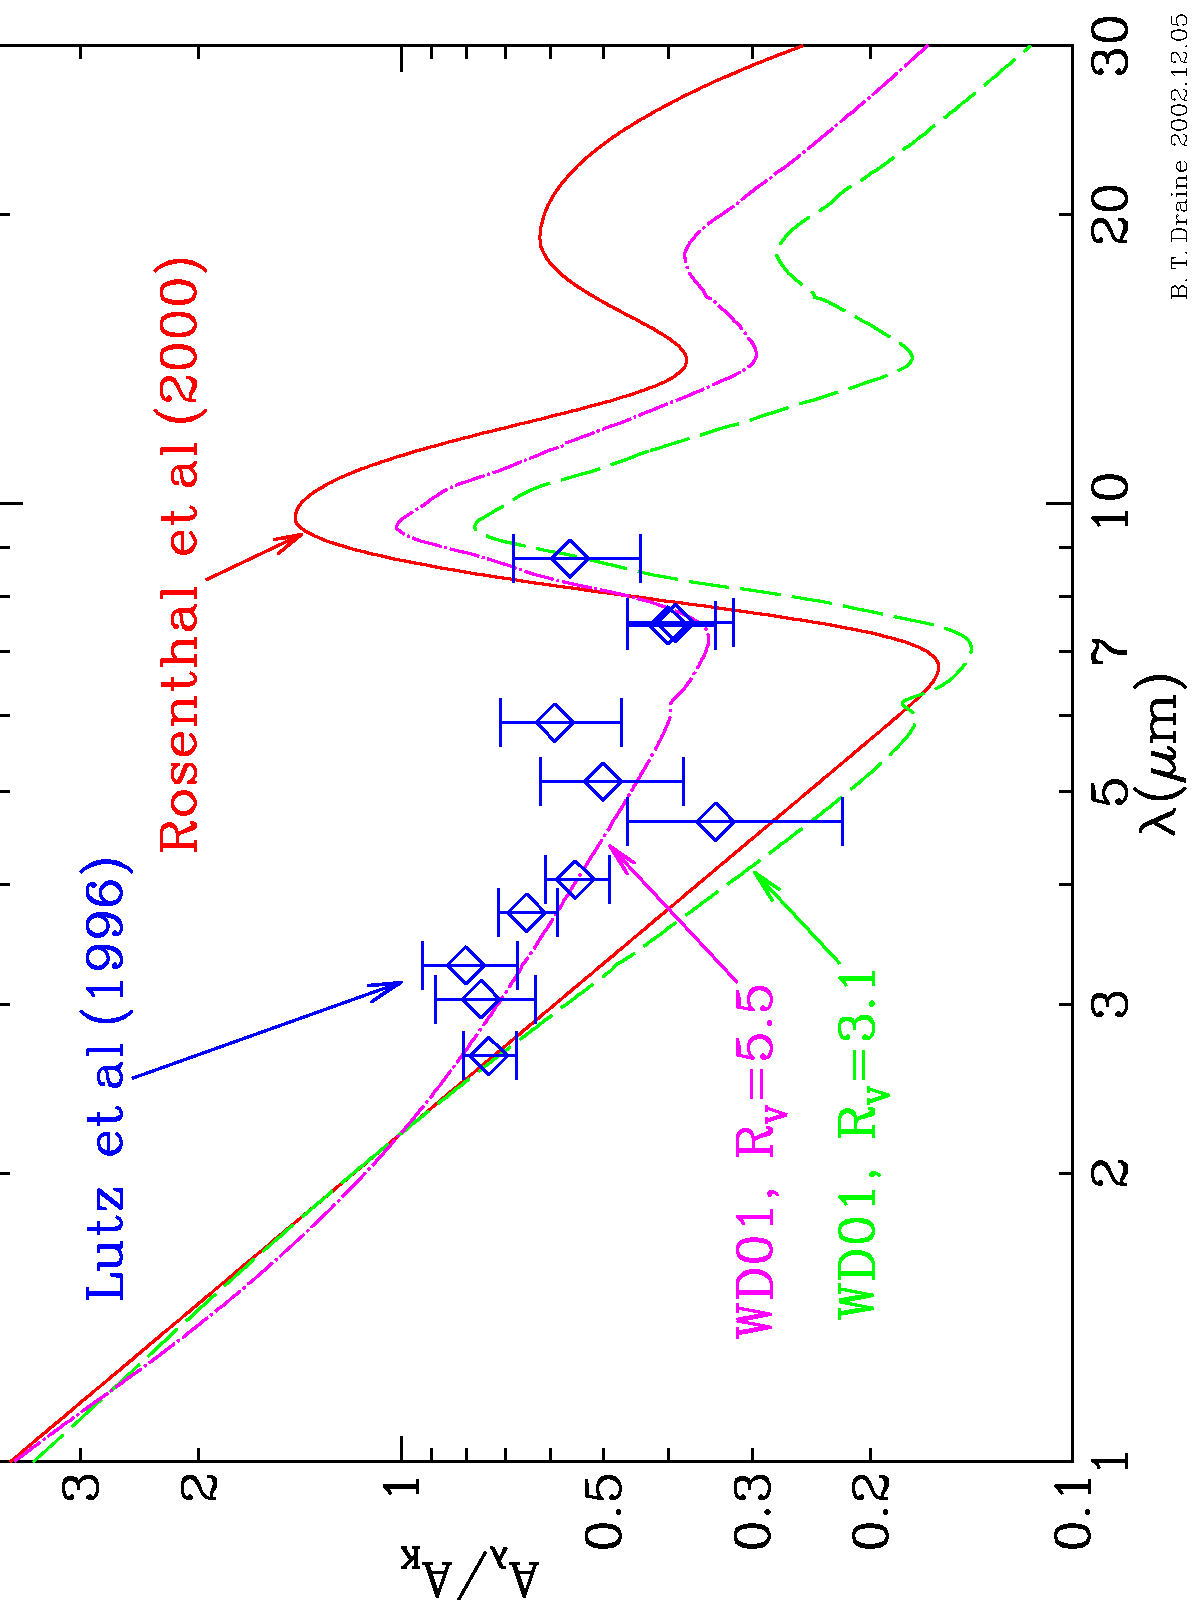
\includegraphics[width=!,height=\textwidth]{./D/draine_araa_f4.pdf}}
\end{center}


\end{frame}


\begin{frame}\frametitle{Uncertainties in $A_\lambda$}

\begin{wrapfigure}{l}{0.56\textwidth}
\includegraphics[width=0.55\textwidth, height = !]{./D/dwek_fig1.jpg}
\end{wrapfigure}  Dwek (2004, ApJL, 611, 109)
proposes that the excess extinction at $\sim$6~$\mu\mathrm{m}$ is due
to metallic needles (ref. Hoyle \& Wickramasinghe).  {\bf short dash}:
silicates, {\bf long dash}: metallic needles, {\bf dots}: graphite,
{\bf dot-dash}: PAHs, {\bf thin solid}: standard extinction.




\[
\tau(\lambda) = \sum_j \int_0^L\,ds \left[
\int_{a_{\mathrm{min},j}}^{a_{\mathrm{max},j}} da f_j(a)
\kappa_j(\lambda,a) \rho_{d,j}(a,s)\right], ~~\text{with} 
\]
\[
\int_{a_{\mathrm{min},j}}^{a_{\mathrm{max},j}}  f_j(a) = 1.
\]



\end{frame}

\begin{frame}\frametitle{NICER and $A_V$ maps}

Lombardi, Alves, 2001, A\&A 377,1023.

\begin{center}
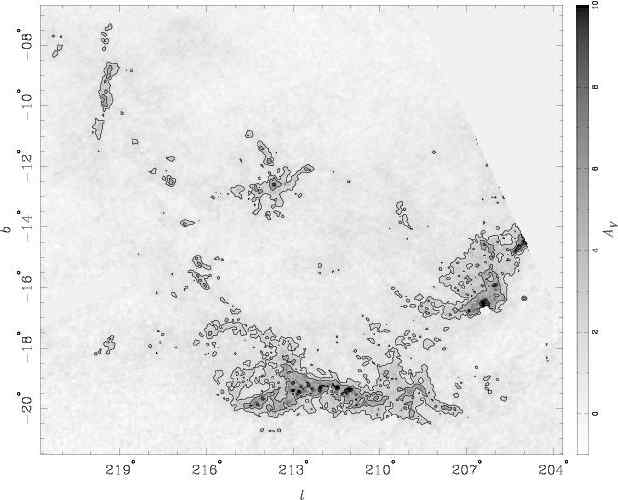
\includegraphics[width=0.6\textwidth,height=!]{./D/lombardi_alves_NICER.jpg}
\end{center}

JHK extinction follows a fairly universal law, so JHK imaging allows
accurate near-IR extinction measurements through stellar counts.

Very useful: $A_V$ can be converted to $N_H$, and thereby to total
masses.


\end{frame}

\begin{frame}\frametitle{The UV bump: VSGs}


\begin{minipage}[t]{0.59\textwidth}
\begin{itemize}
\item The UV bump matches a Lorentzian (in truth a `Drude' profile).
\item The fitting of a Lorentzian allows infering $n_X f_X/ n_H =
9.3~10^{-6}$, and since the oscilator strength of the absorbing specie
  cannot be in excess of $\sim 1$, $f_X \lesssim 0.5$, one requires
  $n_X/n_H \gtrsim 4~10^{-5}$, allowing to consider compounds of
  $\{C,N,O,Mg,Si,Fe\}$.
\item The centre of the bump is constant at  2175\AA,  although the
  width of the bump varies with 1~$\sigma \approx 6\%$.
%\item Grafito podr\'{\i}a explicar  
\end{itemize}
\end{minipage}
\hfill
\begin{minipage}[t]{0.4\textwidth}
\vspace{-1cm}
  \begin{center}
    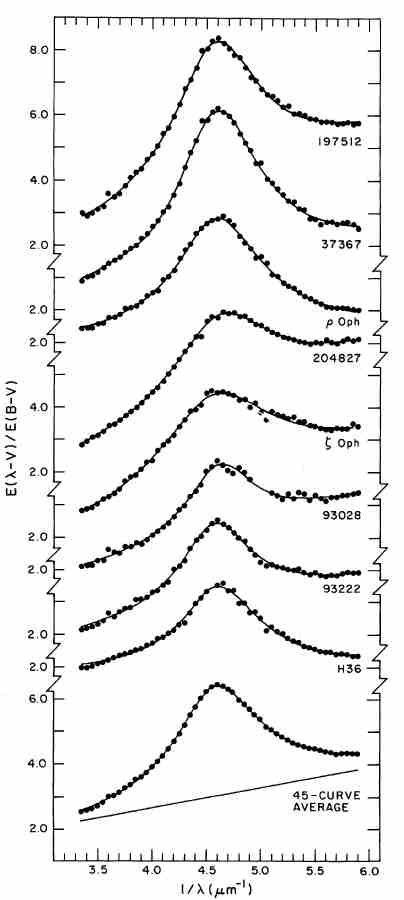
\includegraphics[width=\textwidth,height=!]{./D/uvbump_drude.jpg}
    \end{center}
\end{minipage}


\end{frame}
\begin{frame}\frametitle{}


\begin{minipage}[t]{0.5\textwidth}
\begin{itemize}
\item A ground state transition in the delocalized electrons of the
hexagonal benzene rings lies precisely at 2175\AA.

%\item un transici\'on al nivel excitado en los electrones
%deslocalisados de los anillos hexagonales de benzeno esta precisamente
%a 2175\AA.

\item Graphite, with  $f = 0.16$ could explain  $\lambda_\circ$, and
the absorption strength with C/H$=5.8~10^{-5}$ (OK for cosmic
abundances), but not the FWHM variations. 

\item Variations in the mixture of different PAHs molecules are
required to explain the $FWHM$ variations. 
\end{itemize}
\end{minipage}
\hfill
\begin{minipage}[t]{0.49\textwidth}
\vspace{-0.1cm}
  \begin{center}
\rotatebox{-90}{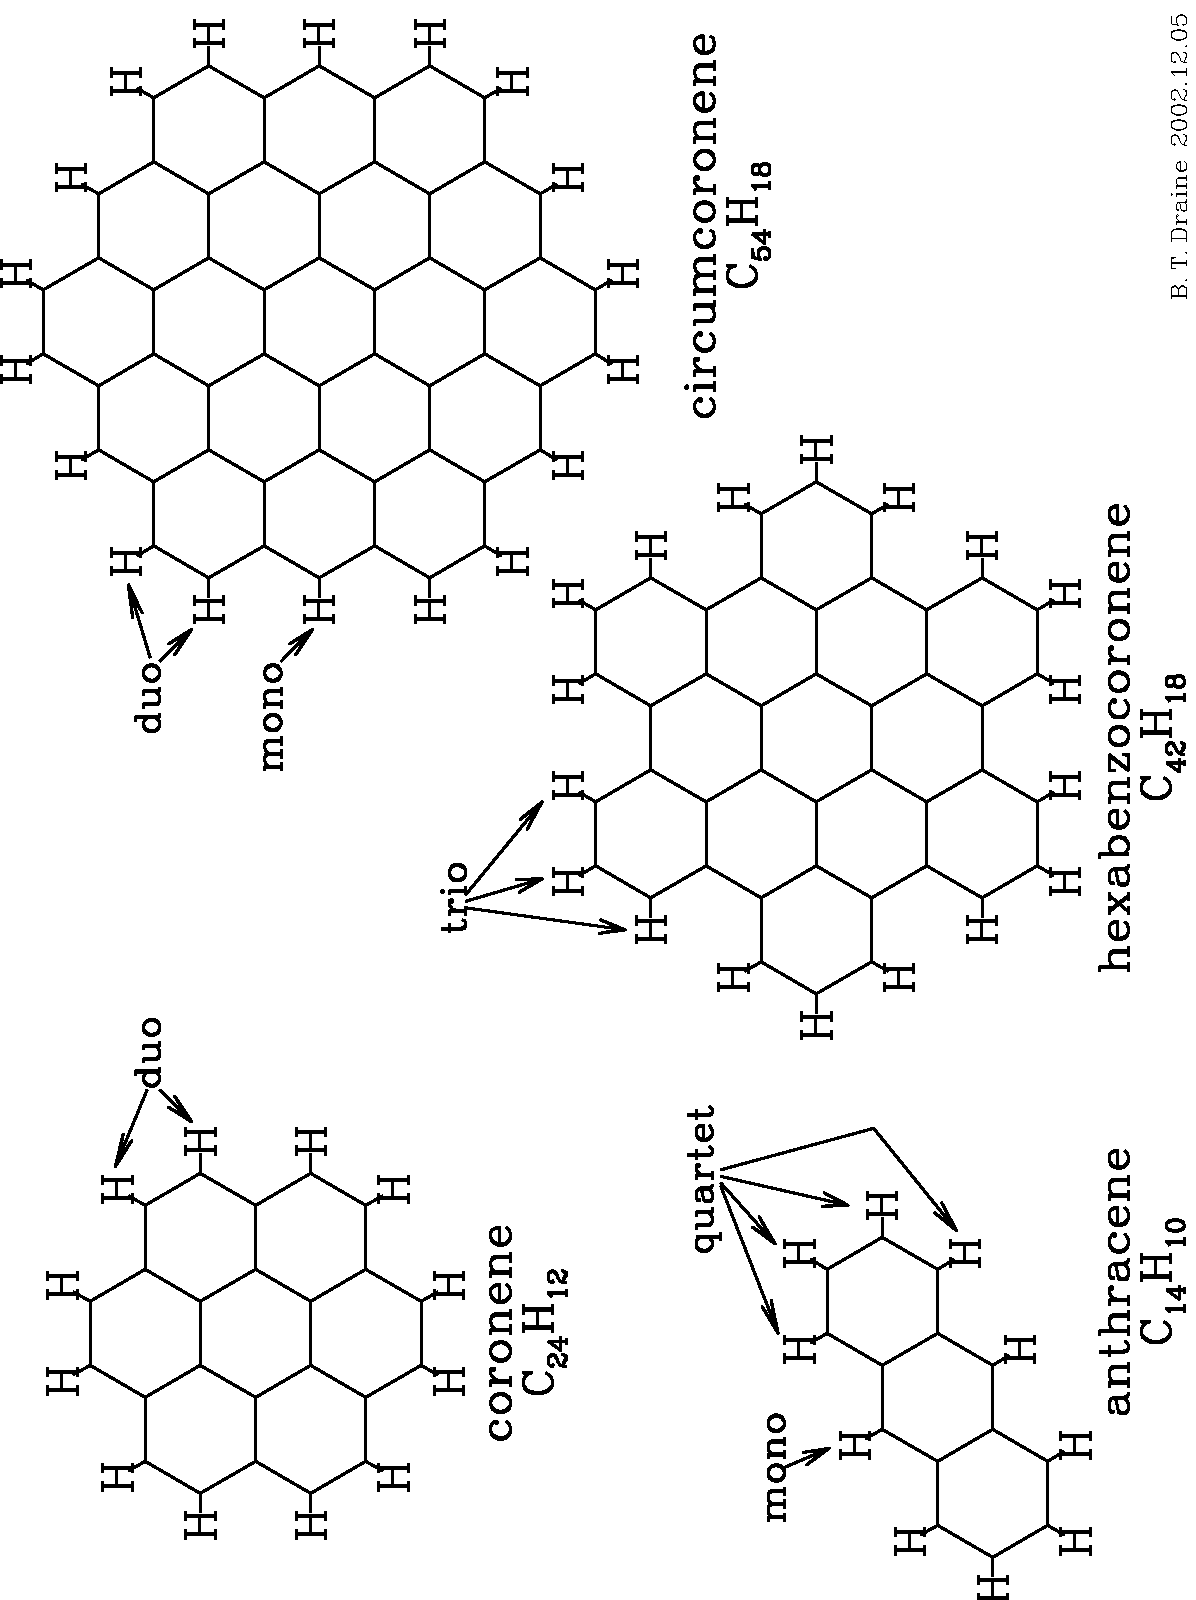
\includegraphics[width=!,height=0.6\textwidth]{./D/draine_araa_f7.pdf}}
    \end{center}
\end{minipage}


\end{frame}
\begin{frame}\frametitle{Silicate extinction}

\begin{itemize}
\item The 10$\mu$m silicate feature is seen in absorption when the
  screen is colder than the background illuminating source. It is seen
  in emission in M stars (C/O$>1$) , or in planetary nebulae with
  C/O$>1$.

\item Stretching  mode of  Si-O at 9.7~$\mu$m. 

\item Properties of silicates vary substantially with environment.

\item The extinction curve at  10$\mu$m is smooth and shows no fine
structure, in marked contrast with the crystalline silicate spectra
$\Rightarrow$ interstellar silicates are amorphous.

\item But there is a significant fraction of crystallinity in
circumstellart disks and AGB (M) star outflows.

\item Bowey et al. propose that up to  60\% of  silicate mass in dense
dark cloud is crystalline (criticised). 
\end{itemize}

 
\end{frame}
\begin{frame}\frametitle{\footnote{Bowey \& Adamson 2002, MNRAS, 334, 94}}

\begin{minipage}[t]{0.3\textwidth}
\vspace{0.5cm}
  \begin{center}
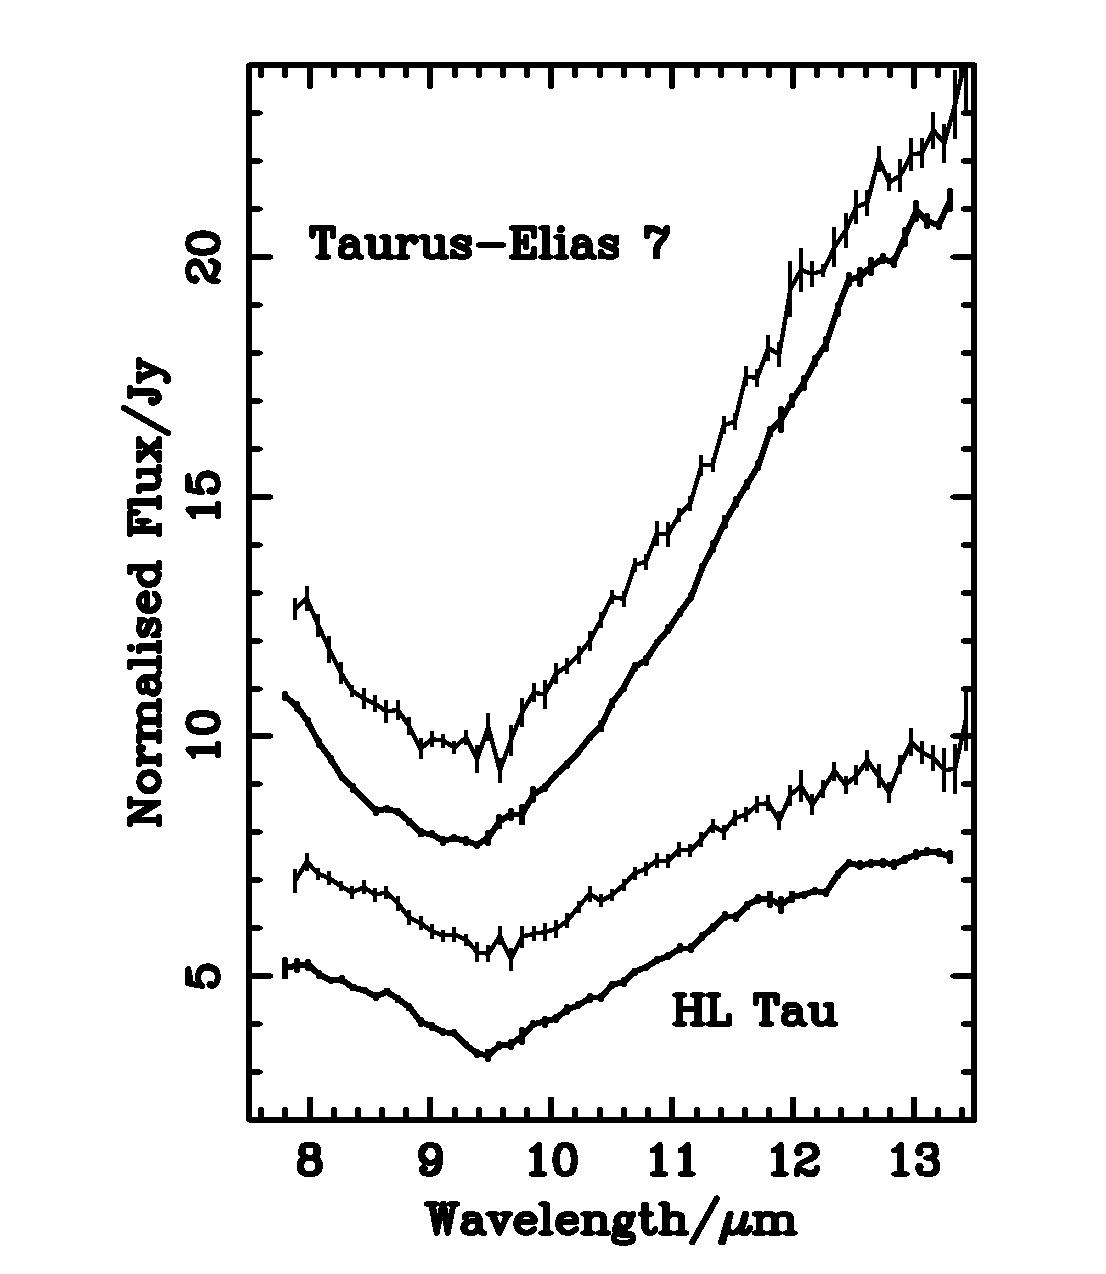
\includegraphics[width=\textwidth,height=!]{./D/bowey_spectra.jpg}
    \end{center}
\end{minipage}
\hfill
\begin{minipage}[t]{0.3\textwidth}
\vspace{-1.0cm}
  \begin{center}
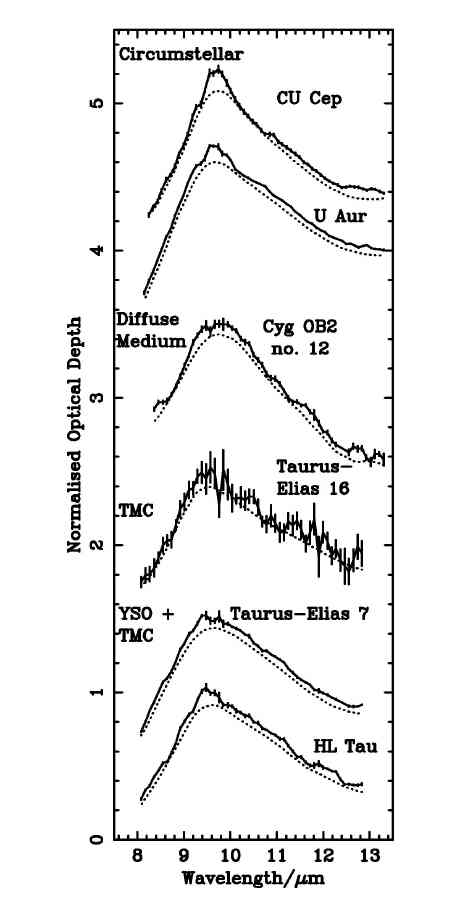
\includegraphics[width=\textwidth,height=!]{./D/bowey_obs_taus.jpg}
    \end{center}
\end{minipage}
\begin{minipage}[t]{0.3\textwidth}
\vspace{-1.0cm}
  \begin{center}
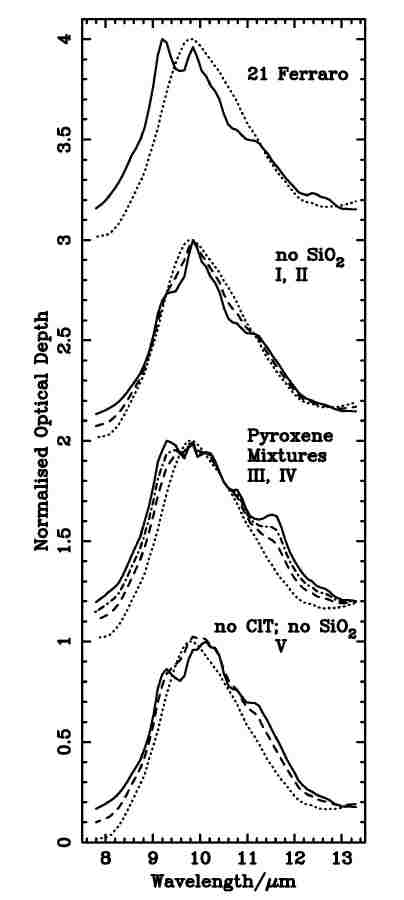
\includegraphics[width=\textwidth,height=!]{./D/bowey_mod_taus.jpg}
    \end{center}
\end{minipage}
\hfill



\end{frame}
\begin{frame}\frametitle{Silicate extinction}
 


\begin{center}
      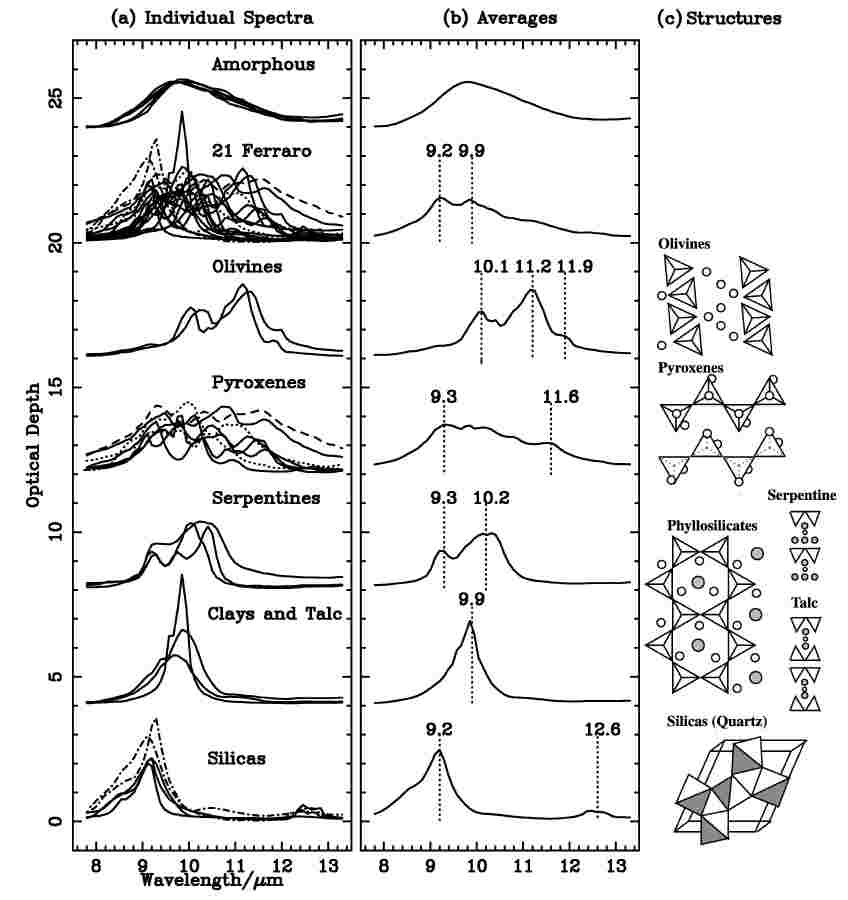
\includegraphics[width=0.6\textwidth,height=!]{./D/cristsil_bowey.jpg}
\end{center}


\end{frame}
\begin{frame}\frametitle{Variations in the silicate profiles\footnote{Van Dischoeck, 2004, AR\&AA}}

\begin{center}
      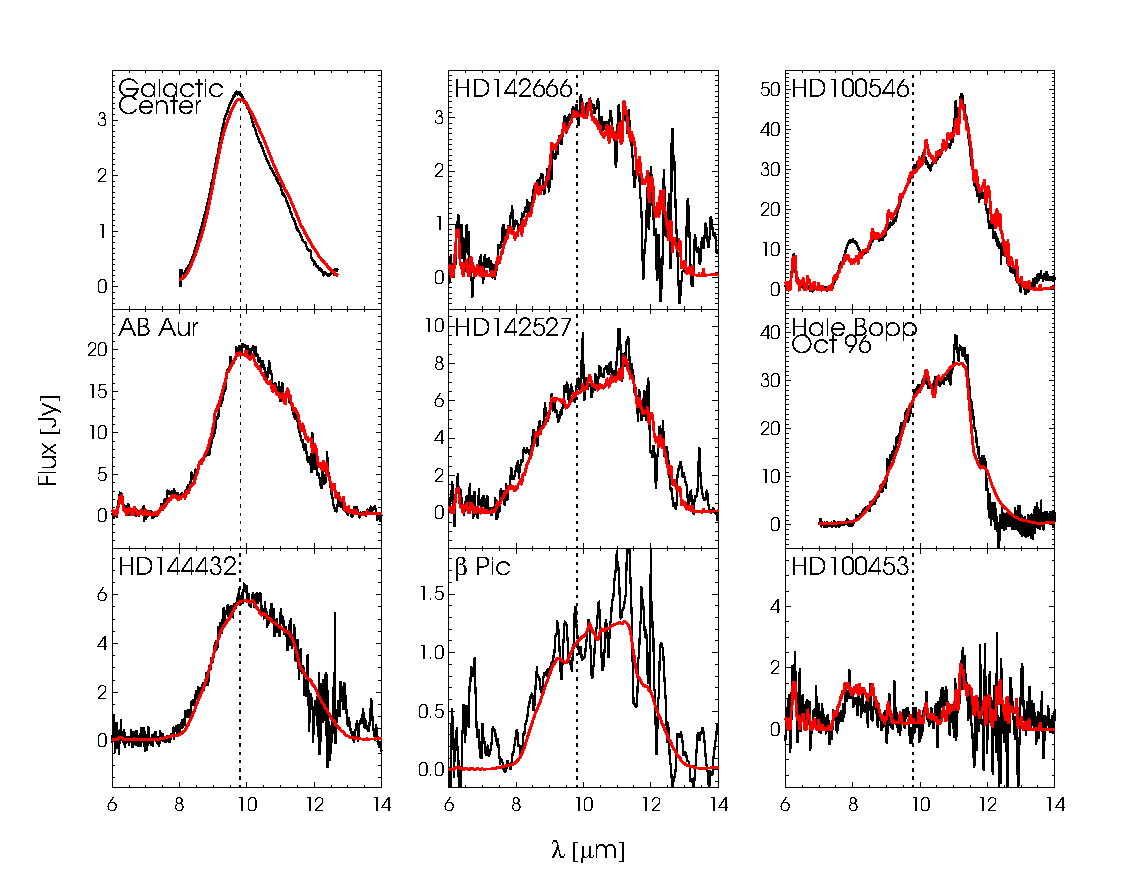
\includegraphics[width=0.9\textwidth,height=!]{./D/dishoeck_fig12.pdf}
\end{center}

\end{frame}
\begin{frame}\frametitle{Absence of crystalline silicates in the diffuse ISM\footnote{Kemper et al. ApJ 2004, 609, 826}}

\begin{minipage}[t]{0.5\textwidth}
\vspace{0.5cm}
  \begin{center}
      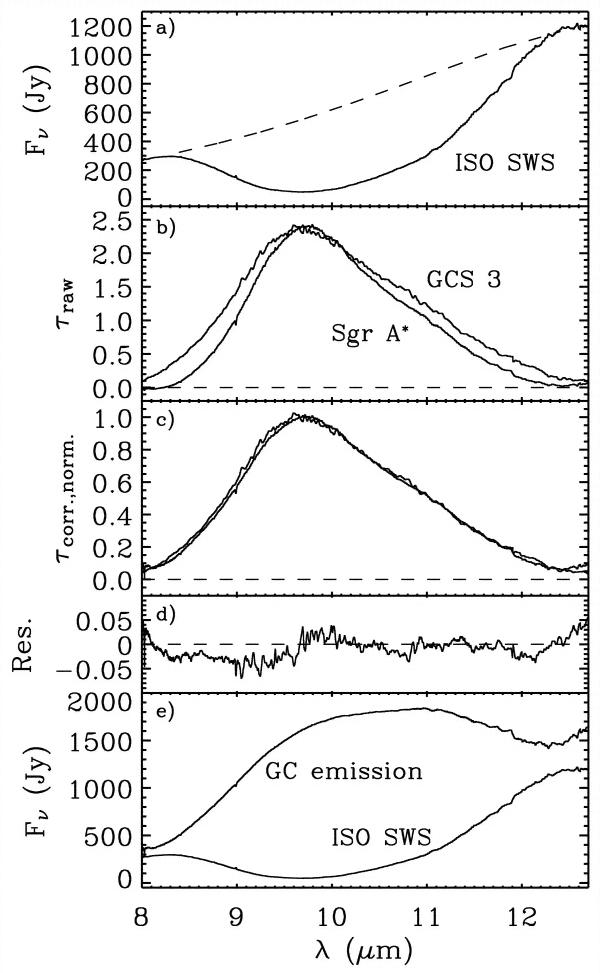
\includegraphics[width=0.6\textwidth,height=!]{./D/taus_ISO_GC.jpg}
      \end{center}
\end{minipage}
\hfill
\begin{minipage}[t]{0.49\textwidth}
\vspace{-0.5cm}
  \begin{center}
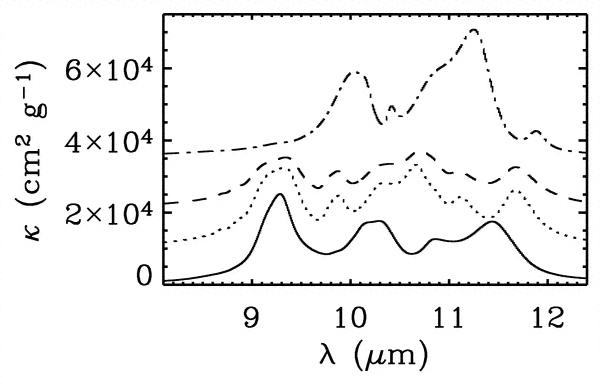
\includegraphics[width=\textwidth,height=!]{./D/crist_ks.jpg}
    \end{center}
$\Rightarrow$ Crystalline silicates represent $\sim~0.2\pm0.2$ by
mass. \\
Since the silicates in the AGB star outflows have high
fractions of crystallinity, there must be substantial interstellar
processing of dust in the ISM.
\end{minipage}


\end{frame}
\begin{frame}\frametitle{Ice absorption}


\begin{center}
\rotatebox{-90}{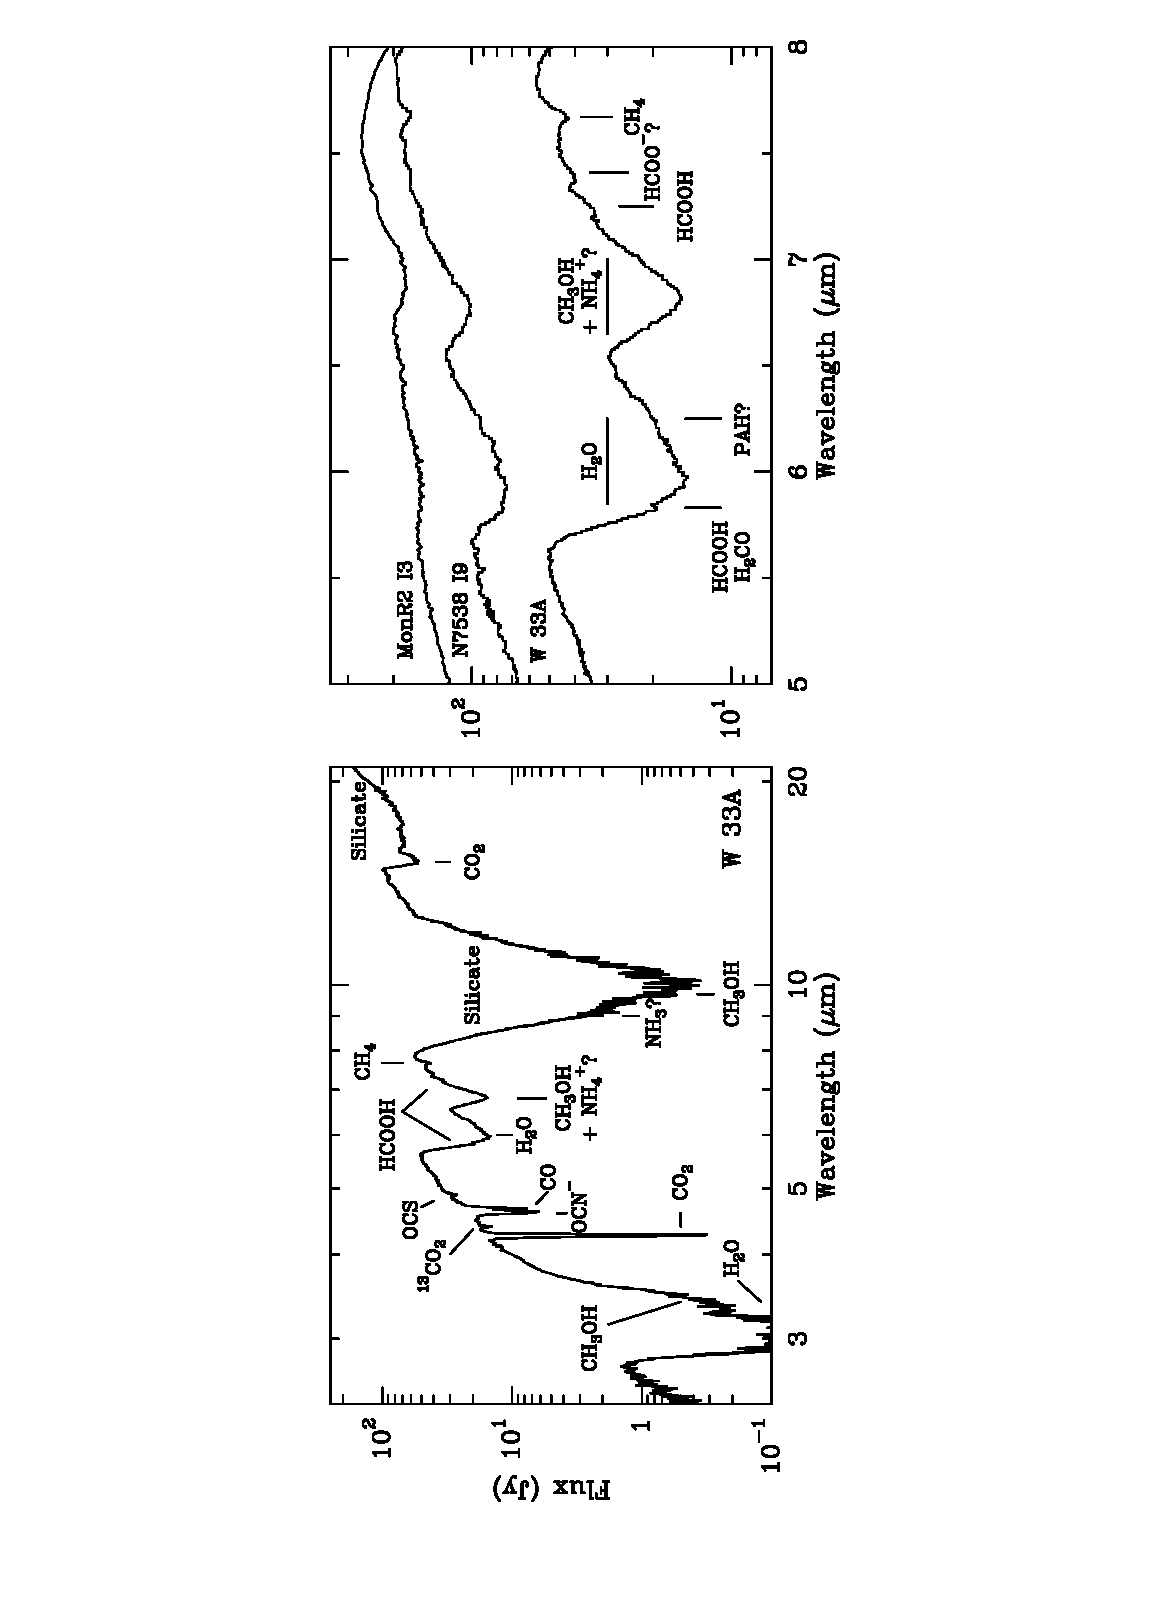
\includegraphics[width=!,height=\textwidth]{./D/dishoeck_fig7.pdf}}
\end{center}









%\foilhead{}
%\leftheader{}
%
%\begin{center}
%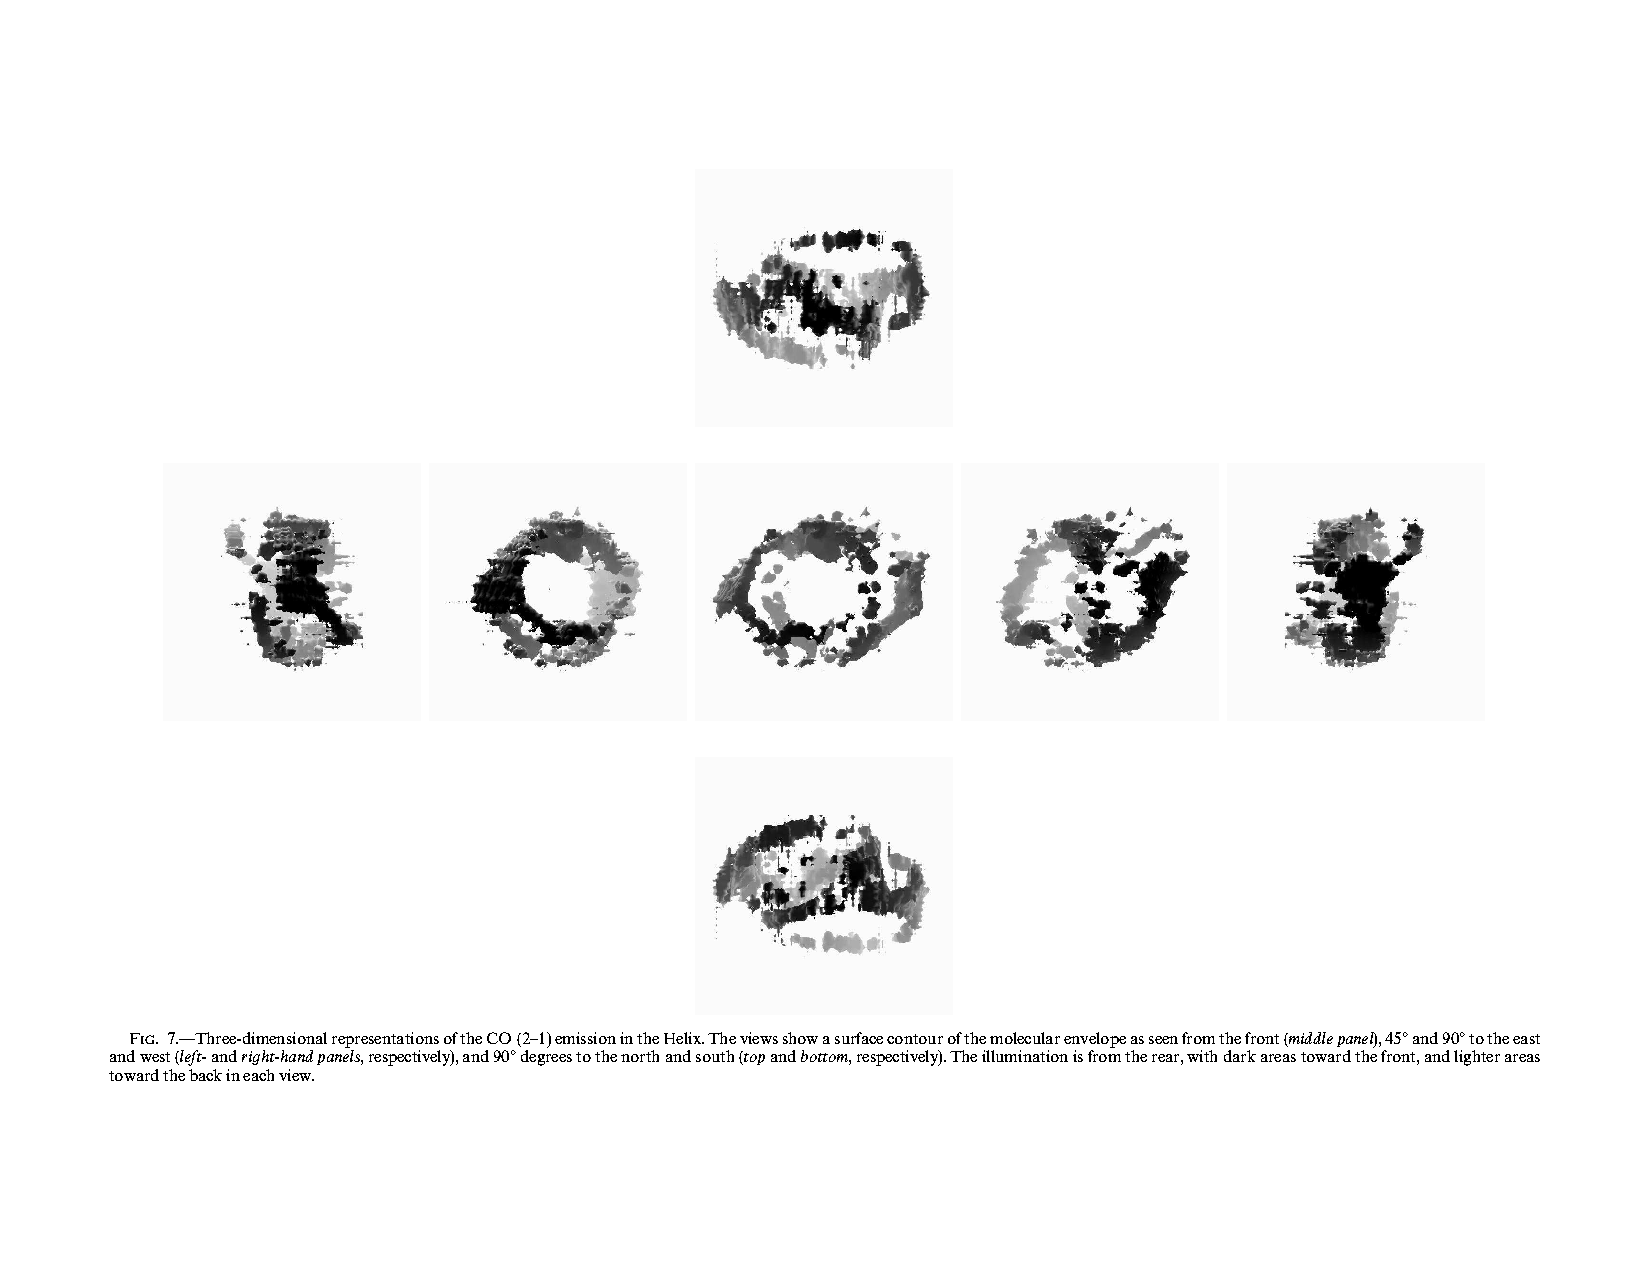
\includegraphics[width=\textwidth,height=!]{./D/ngc7293_3D.pdf}
%\end{center}
%




\end{frame}

\section{IR emission from dust}

\begin{frame}\frametitle{IR emission from dust}

If the grains are in steady state, their internal energy and
temperature are constant, and the emergent spectrum from a homogeneous
cloud is 
\[ 
I_\nu = B_\nu (T_d) \left[ 1 - \exp(-\tau_d) \right], 
\]
with  $\tau = \kappa(\lambda) \int \rho ds $, and
\[ 
\kappa(\lambda) = \frac{1}{1.4 n_H m_H} \int da \frac{dn}{da}
C_\mathrm{abs}(a,\lambda),
\]
where $\rho$ is the mass density (with gas), and $n(a)$ is the number
density of grains with radii $< a$. Thus the column of mass is 
\[
\int \rho ds \approx \frac{1}{\kappa(\lambda)}
\frac{I_\nu}{B_\nu(T_d)}~.
\]
The opacities $\kappa$ and cross sections $C_\mathrm{abs}$ are
tabulated in the web page of B. Draine: {\tt
http://www.astro.princeton.edu/\~draine/dust/dust.html}.

\end{frame}
\begin{frame}\frametitle{IR emission from dust}


The power absorbed by a grain is 
\[
\left.\frac{dE}{dt}\right|_\mathrm{abs} = \int_0^\infty d\nu u_\nu c
C_\mathrm{abs}(\nu),
\]
and emitted  power  is 
\[
\left.\frac{dE}{dt}\right|_\mathrm{rad} = \int_0^\infty d\nu 4\pi B_\nu
C_\mathrm{abs}(\nu).
\]
We can express $T_s$, the steady state temperature, from 
$\left.\frac{dE}{dt}\right|_\mathrm{abs} =
\left.\frac{dE}{dt}\right|_\mathrm{rad}$, {\bf under the assumption
that collisions do not contribute to the thermal blance}.

But in reality $E$, the internal energy of the grain, and $T$, its
temperature, vary stochastically, and the flutuactions are more
pronouced when $h\nu \sim E$, as is the case for very small
grains. 

%Thus one needs to determine the probability density associated
%to $E$, through a thermal balance. 

\end{frame}
\begin{frame}\frametitle{Feature at   3.4~$\mu$m: C-H 
alifatic stretch (carbon chains)}

\begin{center}
  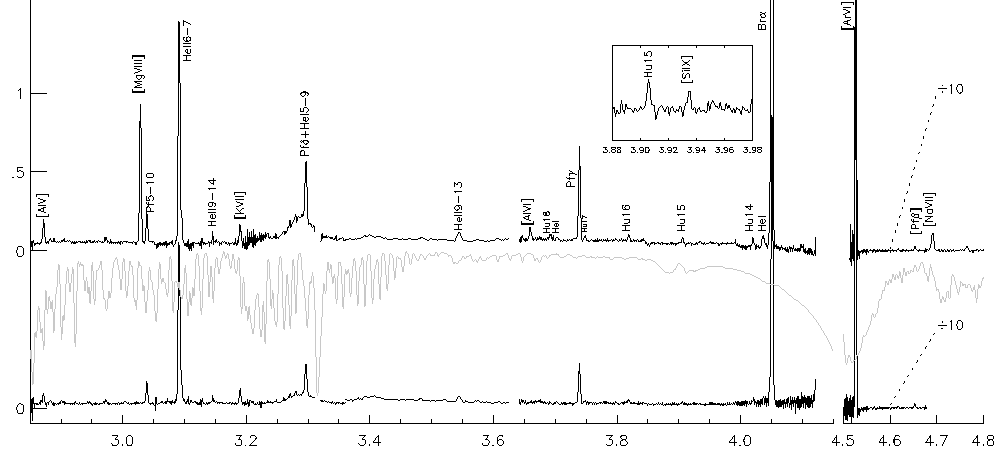
\includegraphics[width=\textwidth,height=!]{./D/specCGS4.pdf}
\end{center}

\end{frame}
\begin{frame}\frametitle{Other dust features}

\begin{itemize}
\item Diamonds are seen in two Herbig AeBe stars and one AGB star,
  through emission bands at 3.4 and 3.5~$\mu$m due to hydrogenated
  surface impurities on an otherwise regular carbon-crystal lattice.

\item SiC (silicon carbide) is seen towards C stars and PNe. 

\item The Extended Red Emission, or a broad featureless continuum at
  6000 to 8000~\AA, is seen towards all lines of sight (i.e. cirrus
  and dark clouds, H\,{\sc ii} regions, PNe and galaxies in
  general). The carriers of ERE have yet to be identified. 


\item Fullerenes (Kroto et al. 1985, Nat, 318, 162) in post-AGB stars and PNe, e.g. Bernard-Salas et al., 2012, ApJ, 757, 41B


\end{itemize}

\end{frame}

\section{VSGs}

\begin{frame}\frametitle{VSGs}



\begin{itemize}

\item  The VSGs are necessary to explain the variations in the UV bump
of the extinction curve.


\item Andriesse (1978) postulated the VSGs to explain the variation of
the dust temperature in a cloud near M17.  $T_\mathrm{colour}$ in the
NIR and FIR are 150K y 38K, respectively, while the NIR and FIR
morphologies are practically identical $\rightarrow$ the two
temperatures are mixed, and it is necessary to postulate the
temperature excursions of VSGs (which were called Platt particles at
the time). 

\item Sellgren et al. (1983) found  that the NIR emission in
reflection nebula is extended and consists at least of one emission
band at 3.3~$\mu$m as well as a continuum with $T_\mathrm{colour} =
1000$~K, with minimal variations with distance from the central star.
Sellgren (1984, ApJ, 277, 623) noted that if the dust was in radiative
equilibrium with the star, its temperature should decrease rapidly
with distance, and so postulated the VSGs.

\end{itemize}

\end{frame}


\begin{frame}\frametitle{VSGs}

\begin{itemize}
\item The  12~$\mu$m and 25~$\mu$m emission from Galactic cirrus, 
discovered by {\em IRAS}, is much higher than that expected from large
grains in equilibrium with the local radiation field (with T$\sim
18-25~$K, Boulanger \& Perault 1988).

\item Spinning dust?

\end{itemize}

\end{frame}
\begin{frame}\frametitle{Stochastic heating of VSGs}


\begin{center}
\rotatebox{-90}{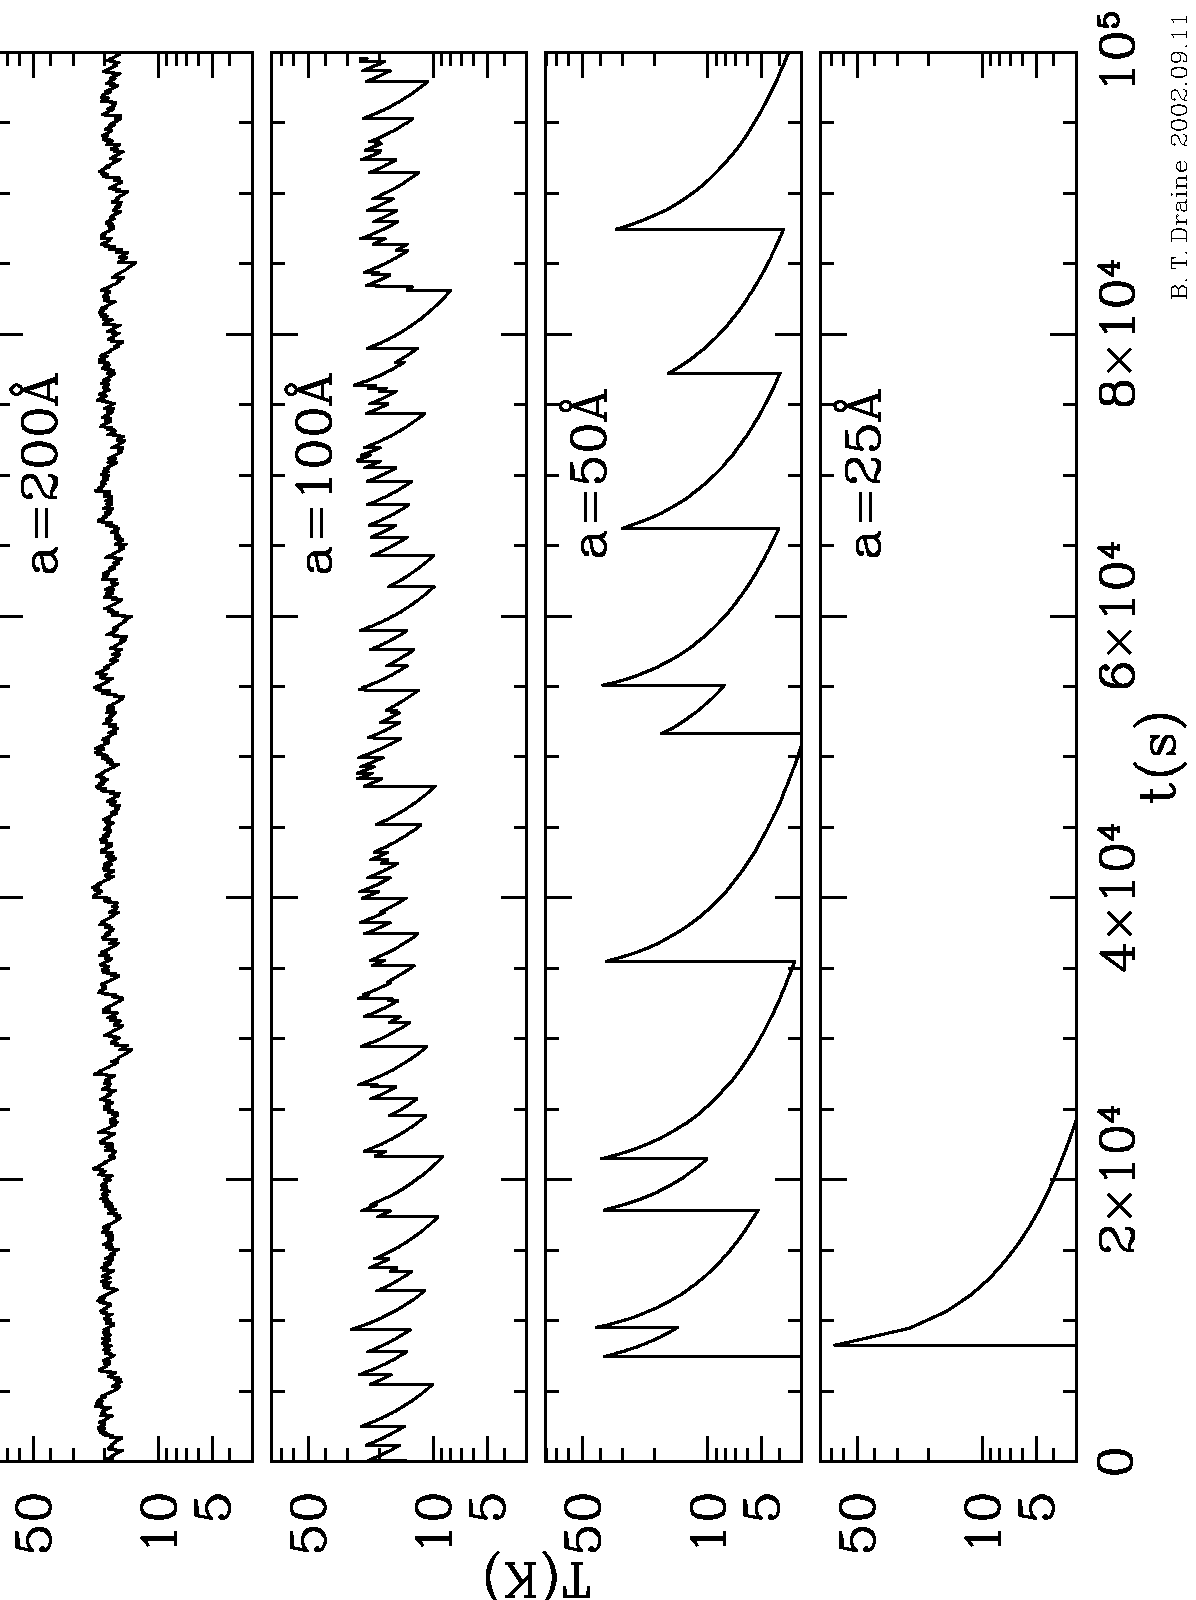
\includegraphics[width=0.5\textwidth,height=!]{./D/T_fluctuations.pdf}}
\end{center}

A grain with radius $5$~\AA (i.e. a PAH) receives 1 UV photon (10~eV)
per year in the radiation field of the solar neighbourhood. When
absorption occurs, the dust grain temperature may rise up to 1000~K.
  

%\begin{floatingfigure}{16cm}
%\includegraphics[width=15cm,height=!]{dwek_fig1.jpg}
%\end{floatingfigure} 

\end{frame}
\begin{frame}\frametitle{}

\begin{minipage}[t]{0.55\textwidth}
\vspace{-0.5cm}
The state of the art in calculations of the VSG emissivity is that by
Draine \& Li (2001, ApJ, 551, 807), who estimated the quantized energy
levels of the VSGs and their corresponding transition rates. See also
Draine \& Anderson (1985, 292, 494), D\'esert et al. (1986, A\&A, 160,
295), Guhathakurtha \& Draine (1989, ApJ, 345, 230).  \\

The problem involves modelling grains as discrete systems, where the
rate of upwards transitions are \[ T_{l\rightarrow u} =
C_\mathrm{abs}(E_u - E_l) c \frac{u_E}{E_u - E_l} \Delta E_u,\] and
$T_{u\rightarrow l}$ is obtained by detailed balance.

\end{minipage}
\hfill
\begin{minipage}[t]{0.4\textwidth}
%\vspace{-1cm}
\begin{center}
\vspace{0.5cm}
%\rotatebox{-90}{\includegraphics[width=!,height=15cm]{./P_E.pdf}}
\includegraphics[width=\textwidth,height=!]{./D/P_E.pdf}
\end{center}
\end{minipage}


\end{frame}
\begin{frame}\frametitle{}


The probability density $P(E)$ in a discretized grain is then obtained
by solving:
\[
\frac{d}{dt} P_i = \sum_{j\ne i} T_{ij} P_j -  \sum_{j \ne i} T_{ji} P_i.
\]


Given  $P(E)$, the power density emitted by a single grain is 
\[
S_\lambda = 4 \pi \int dE \frac{dP}{dE} C_\mathrm{abs}(\lambda)
B_\lambda(T(E)).\]

The temperature of the grain can be defined assuming the energy of the
grain is equal to its expectation value, for a vibrational system in
contact with a heat bath:
\[
\langle E \rangle =  \sum_j  \frac{\hbar \omega_j
}{\exp(\hbar\omega_j/kT) -1},
\]
where the sum extends over all normal modes.

\end{frame}
\begin{frame}\frametitle{}


It is reasonable to apply thermodynamics to a single molecule, say
coronene (C$_{24}$H$_{12}$), because it has $~10^{22}$ vibrational
states with energies inferior to 1~eV $\Rightarrow 1/T=
\partial S / \partial E$, in the canonical ensemble.  

% and it is possible to calculate  $E(S,V,N)$.

The function $P(E)$ depends on each astrophysical situation, but the
only calculations available apply to the diffuse ISM.

\end{frame}
\begin{frame}\frametitle{}


\vspace{-1cm}
\begin{center}
%\rotatebox{-90}{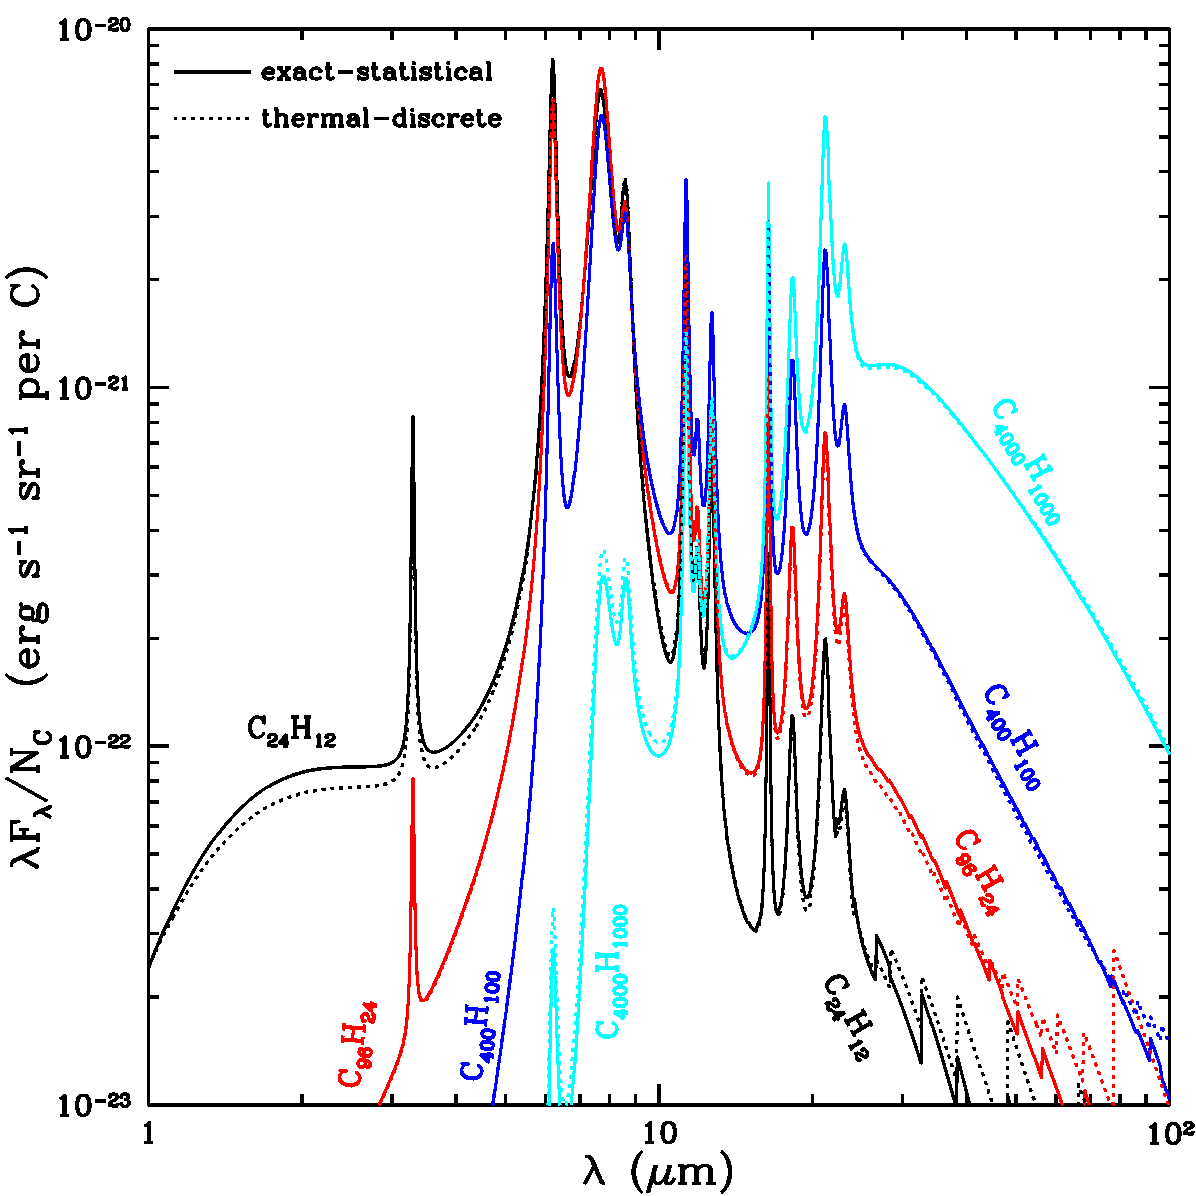
\includegraphics[width=!,height=15cm]{./D/draine_li_f14.pdf}}
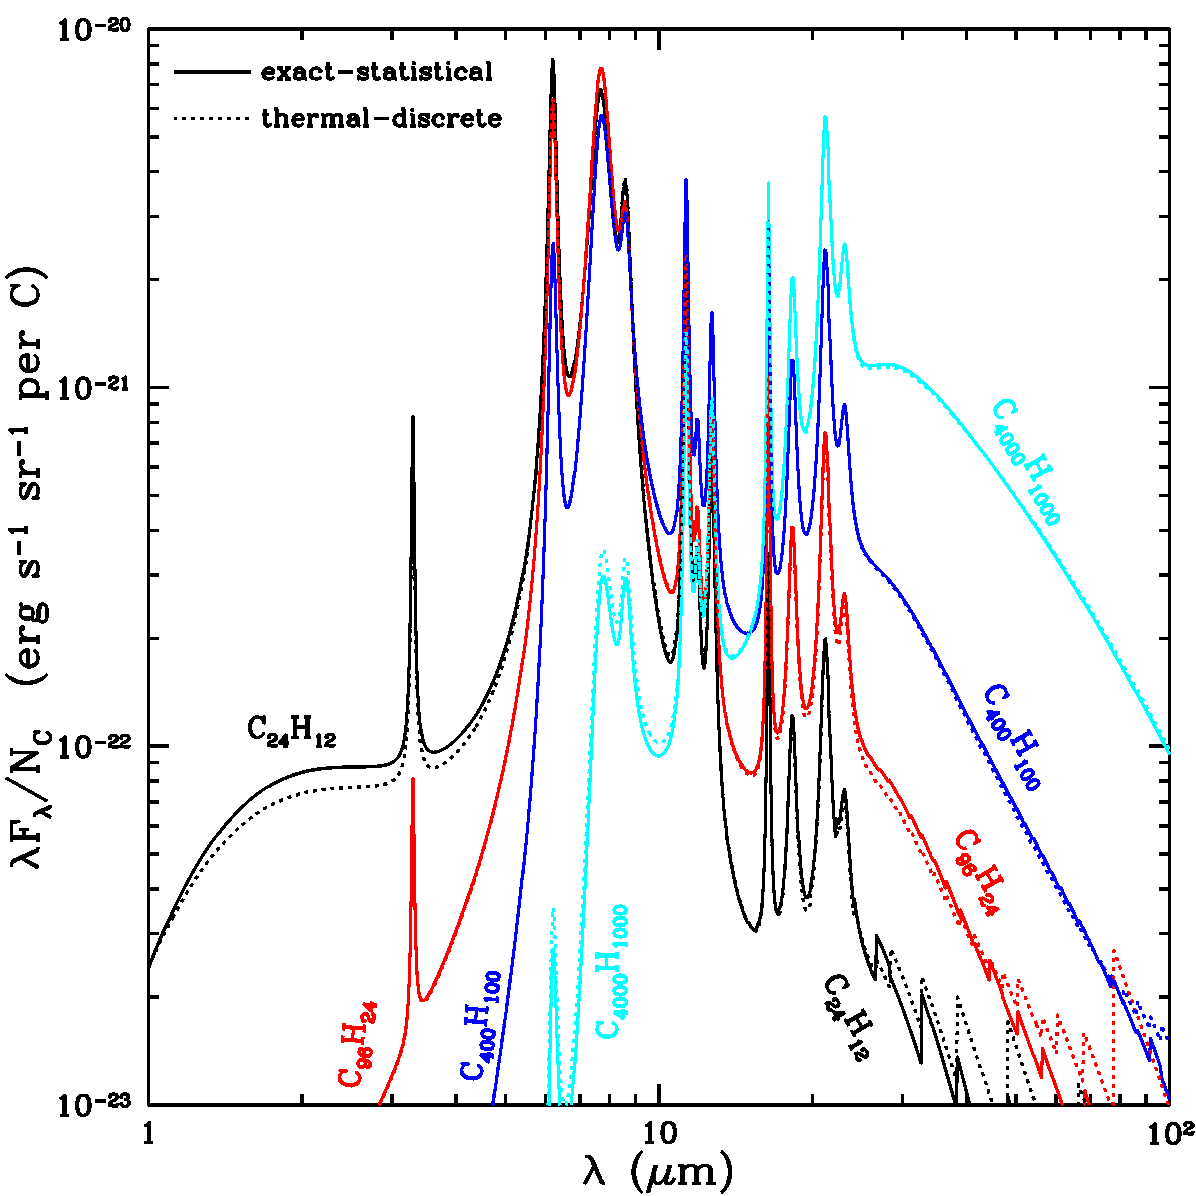
\includegraphics[width=!,height=0.7\textwidth]{./D/draine_li_f14.pdf}
\end{center}

\end{frame}
\begin{frame}\frametitle{}


\vspace{-1cm}
\begin{center}
\rotatebox{-90}{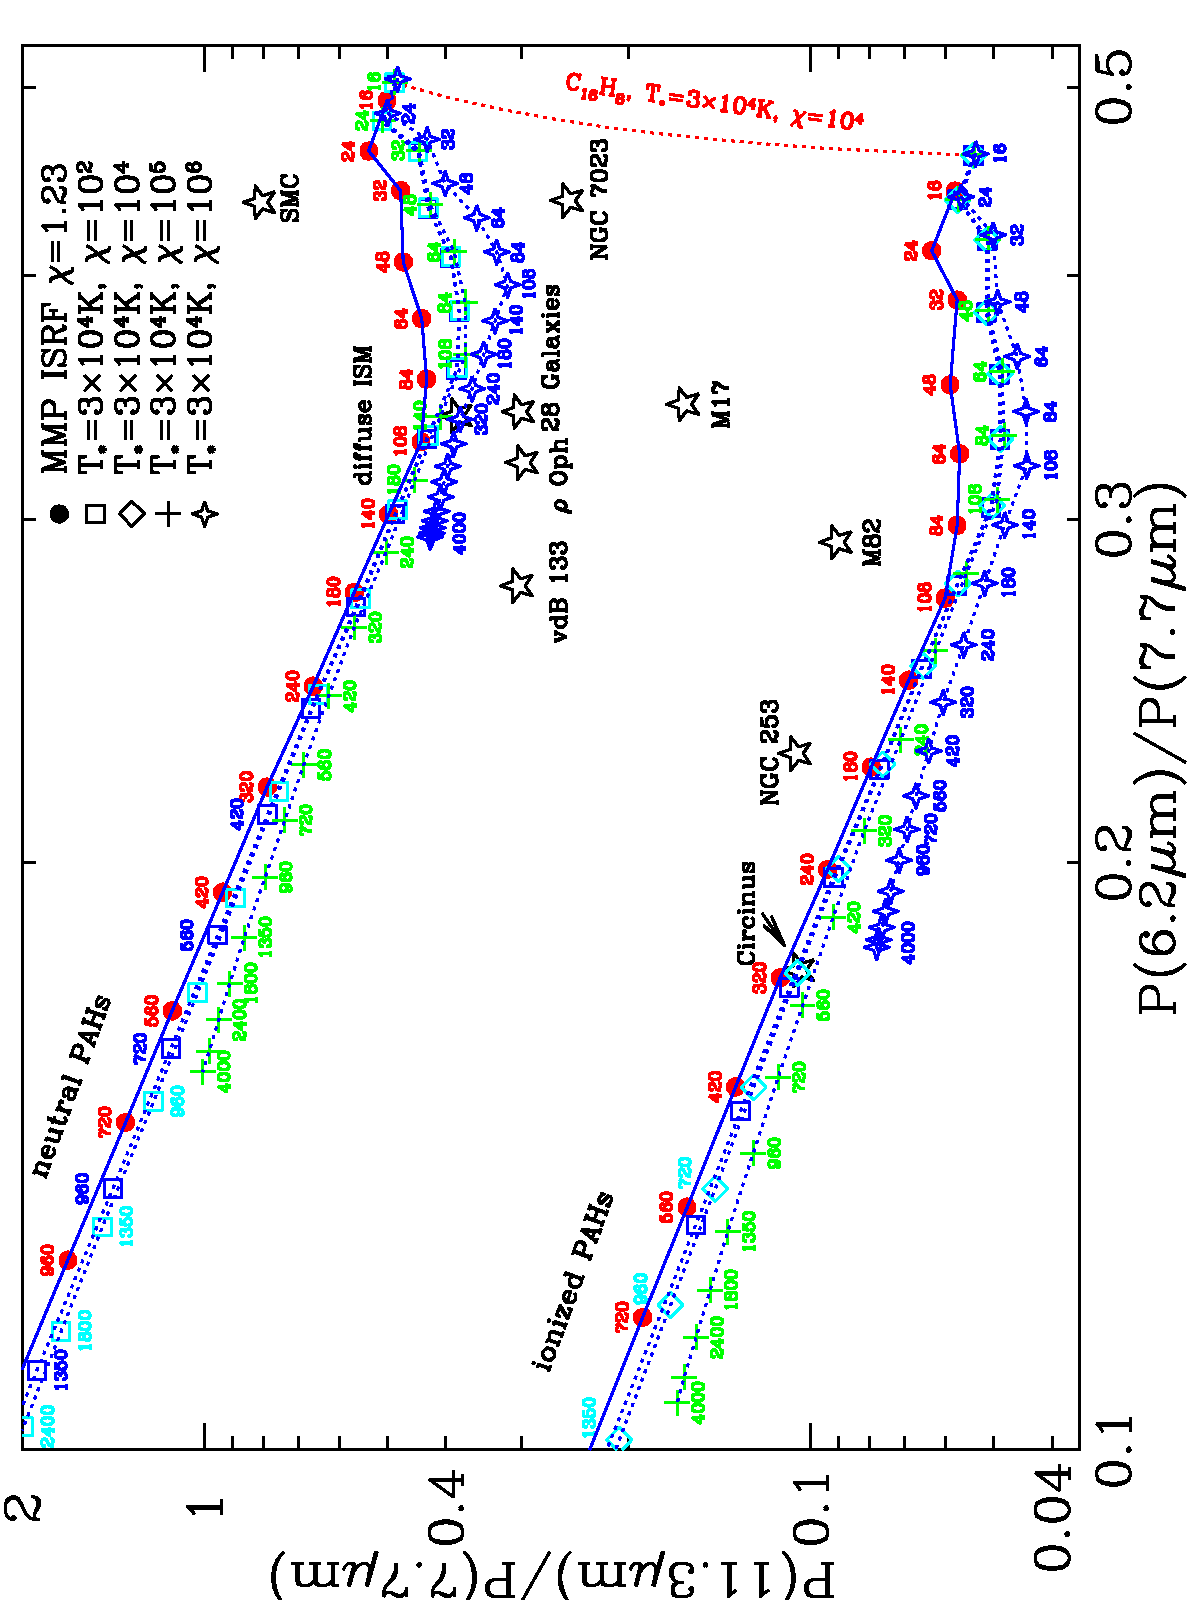
\includegraphics[width=!,height=0.7\textwidth]{./D/draine_li_f16.pdf}}
\end{center}

\end{frame}

\section{The cycle of interstellar dust}

\begin{frame}\frametitle{Evolution of dust: sources}

\begin{itemize}
\item dust features are observed in red giants.
\item the ``super-wind'' on the AGB phase is very enriched in dust
(AGB stars are conspicuous {\em IRAS} sources).
\item M stars (with O/C $>$ 1 and classified by the presence of molecular lines such as TiO),
show the silicate dust feature at  10$\mu$m.
\item C stars  (with C/O $>$ 1 and classified by the presence of
molecular lines such as CH, C$_2$ y CN), show SiC features and
graphite continuum.
\end{itemize}

The details of the condensation of dust are complex. It is believed
that condensation occurs in ``detashed shells'' of the AGB phase
(shielding from the stellar radiation is required to cool the shell
and condense elements).

\end{frame}
\begin{frame}\frametitle{Condensation
temperatures} 

\begin{center}
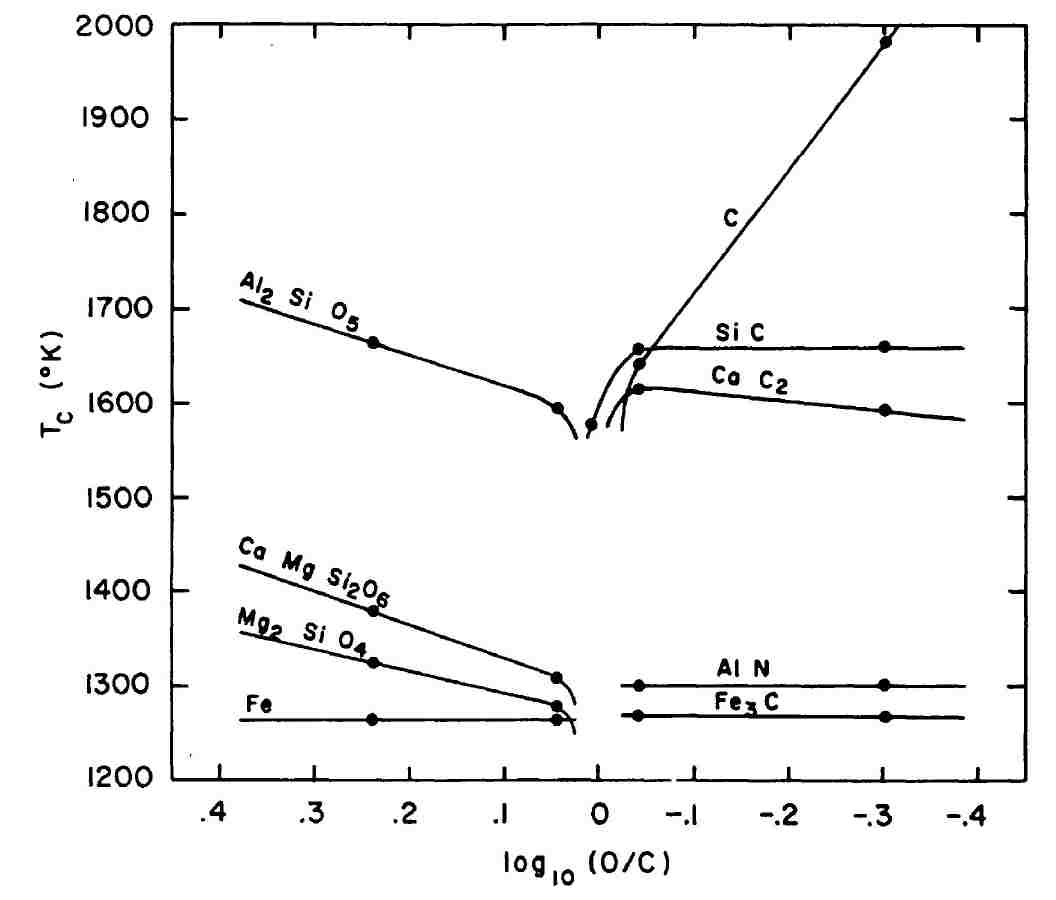
\includegraphics[width=!,height=0.8\textwidth]{./D/Tcond_gilman.jpg}
\end{center}

\end{frame}
\begin{frame}\frametitle{Sources of interstellar dust}

\begin{center}
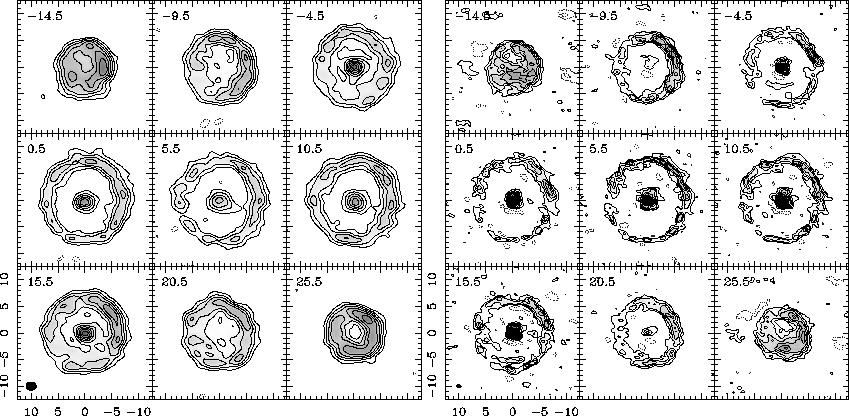
\includegraphics[width=\textwidth,height=!]{./D/thinCOshell.jpg}
\end{center}
CO(1-0) and CO(2-1) in UCameopardalis (Lindqvist et al. 1998, 351, L1)
$\rightarrow$ He-shell flashes modulate the rate of mass loss from
$\sim10^{-7}$M$_\odot~$yr$^{-1}$ to $\sim10^{-5}$M$_\odot$~yr$^{-1}$.

\end{frame}
\begin{frame}\frametitle{AGB stars}

\begin{center}
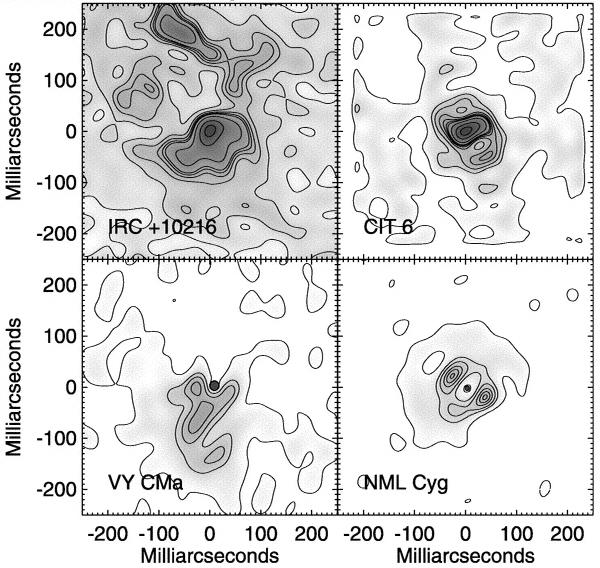
\includegraphics[width=!,height=0.6\textwidth]{./D/irc+10216_iota_1998.jpg}
\end{center}
Monnier et al. (2004, ApJ, 605, 436).

\end{frame}
\begin{frame}\frametitle{Evolution of dust: IRC+10216}

\begin{center}
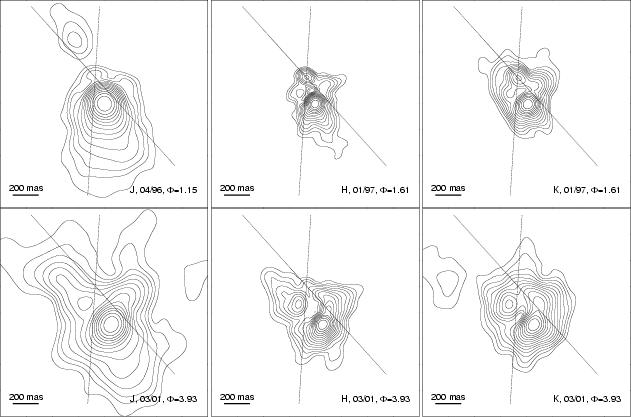
\includegraphics[width=!,height=0.6\textwidth]{./D/irc+10216_evolution.jpg}
\end{center}
Time evolution of the dusty envelope  (Weigelt et al. 2002, A\&A,392,
131).

\end{frame}
\begin{frame}\frametitle{Evolution of dust: the PN phase}

\begin{minipage}[t]{0.5\textwidth}
\begin{center}
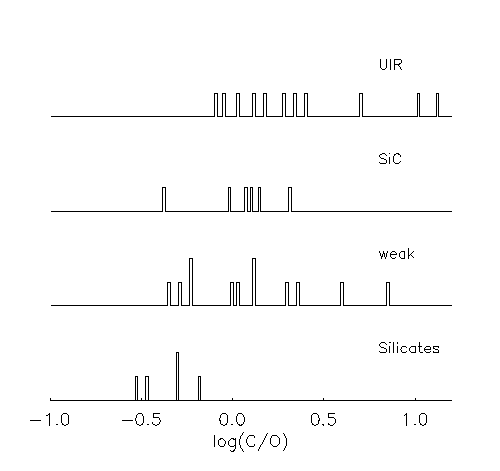
\includegraphics[width=\textwidth,height=!]{./D/dust_CO.pdf}
\end{center}
\end{minipage}
\hfill
\begin{minipage}[t]{0.45\textwidth}
\begin{center}
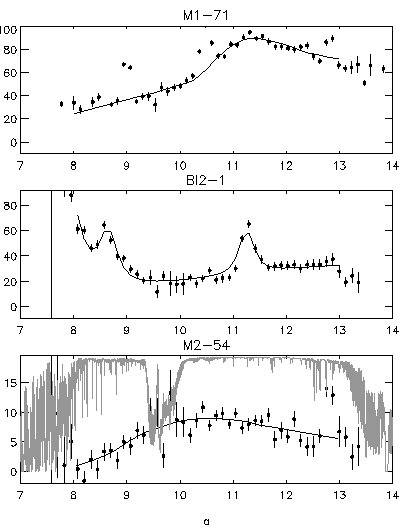
\includegraphics[width=\textwidth,height=!]{./D/10umspecs_ex.pdf}
\end{center}
\end{minipage}

\end{frame}
\begin{frame}\frametitle{Evolution of dust:
the PN phase and the C/O dichotomy}


\begin{center}
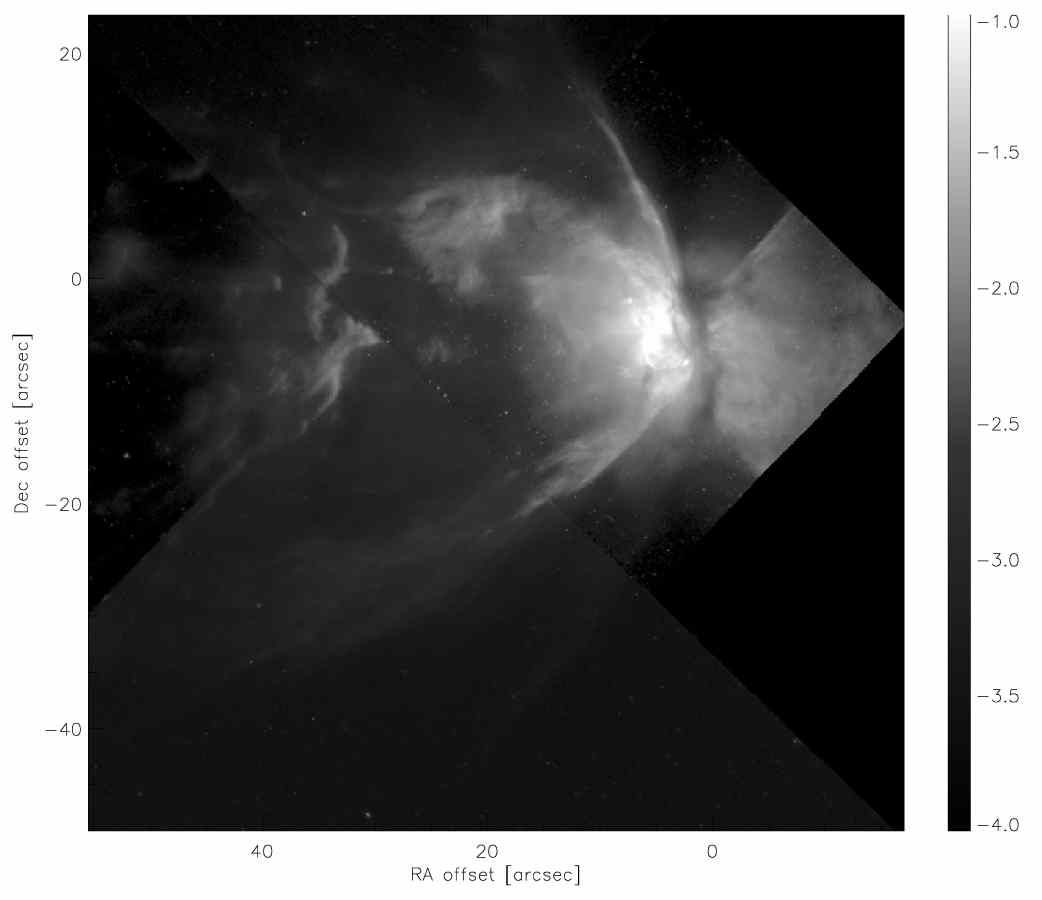
\includegraphics[width=0.8\textwidth,height=!]{./D/matsuura_hstngc6302.jpg}
\end{center}


\end{frame}
\begin{frame}\frametitle{Evolution of dust:
the PN phase and the C/O dichotomy}


\begin{center}
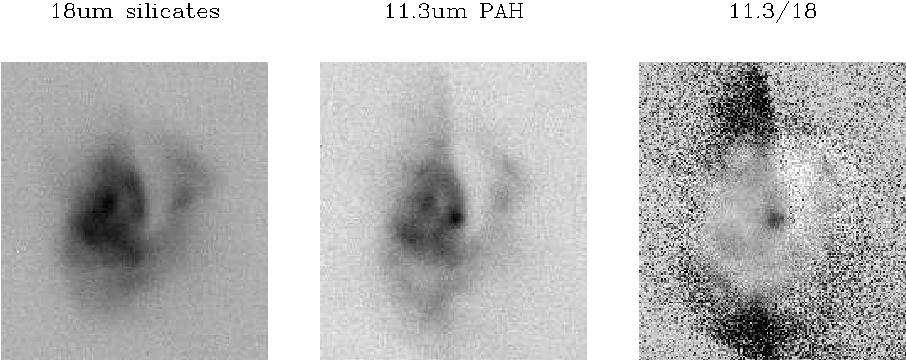
\includegraphics[width=\textwidth,height=!]{./D/trecs_prelim.pdf}
\end{center}


\end{frame}
\begin{frame}\frametitle{Evolution of dust:
SNe as dust factories}

\begin{itemize}
\item Red giants and supergiants are easily indentified as sources of
interstellar dust.  Evolved stars inject dust in the ISM.  But does
circumstellar dust survive the SN event?

\item The sub-mm detection of red-shifted dust from primordial
galaxies (Ivison et al. 2000, MNRAS, 315, 209) implies the efficient
production of dust on very short timescales, such as can only be
provided by type II SNe.


\item Isotopic anomalies in meteoritic inclusions favor the production
  of dust following the SN event (i.e. the SUperNOvaeCONdensates). 

\item The thermal echo due to radiative heating of the dusty winds
from the precursor star (as in SN 1987A, Roche 1989, Nature, 337, 533)
allows a measure of the circumstellar dust mass, and thereby a
constraint on the precursor spectral type. Such a diagnostic is a lot
more difficult from the near-IR spectra (uncertain contribution from
VSGs and other excitation mechanisms).

\end{itemize}.

\end{frame}
\begin{frame}\frametitle{SN~1987A}

Bouchet et al. (2004, ApJ, 611, 394) found a mid-IR source in
SN~1987A, at the location of the SN ejecta, with about
$10^{-3}$~M$_{\odot}$ in dust.
\vspace{-0.1cm}
\begin{center}
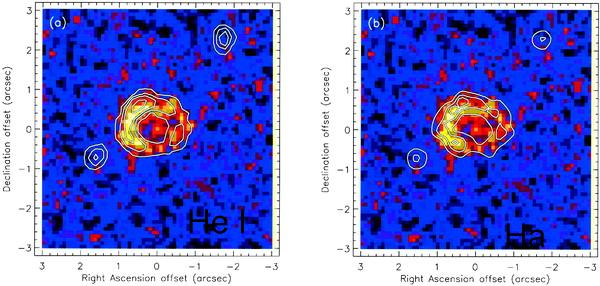
\includegraphics[width=0.5\textwidth,height=!]{./D/SN1987A_1.jpg}
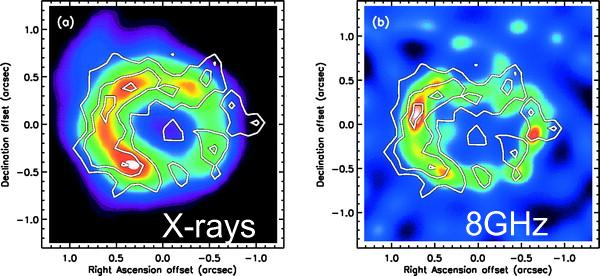
\includegraphics[width=0.5\textwidth,height=!]{./D/SN1987A_2.jpg}
\end{center}
\vfill


\end{frame}
\begin{frame}\frametitle{SN~1987A}

\begin{center}
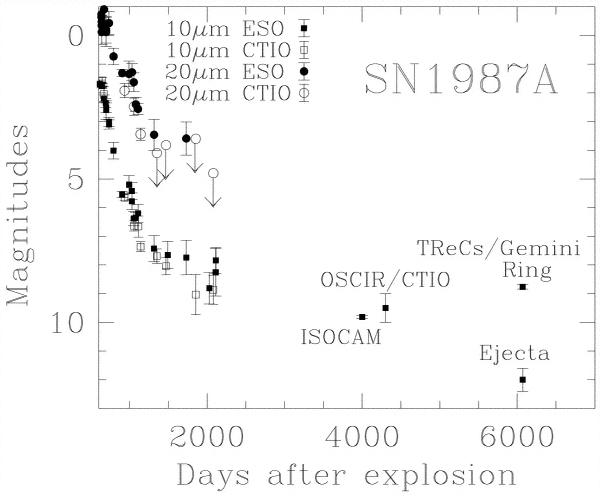
\includegraphics[width=0.5\textwidth,height=!]{./D/SN1987A_lightcurve.jpg}
\end{center}
\vfill The ejecta detected by Bouchet et al. corresponds to the
exponentially decaying mid-IR lightcurve. The equatorial ring is
currently heated by the collision of the supernova blast on
circumstellar shell.

\end{frame}
\begin{frame}\frametitle{SN~2002hh: first IR echo since SN~1987A.}



%\begin{center}
%\includegraphics[width=15cm,height=!]{./barlow_sn2002hh_fig1.jpg}
%\end{center}
%\vfill


\begin{minipage}[t]{0.5\textwidth}
\vspace{0.5cm}
\begin{center}
\includegraphics[width=\textwidth,height=!]{./D/barlow_sn2002hh_fig1.jpg}
\end{center}
\end{minipage}
\begin{minipage}[t]{0.48\textwidth}
\vspace{-0.5cm}
\begin{itemize}
\item (a, b) SINGS IRAC 5.8 and 8.0 $\mu$m images of a 30''x29'' region
   around SN 2002hh (1.1'' per pixel), obtained on 2004 June 10.

\item (c) SINGS MIPS 24$\mu$m image of the same region ( 2.6'' per
   pixel), obtained on 2004 July 9.

\item (d) Gemini North Michelle 11.2$\mu$m image of SN 2002hh (0.099''),
   obtained on 2004 September 26.
\end{itemize}
\end{minipage}


\end{frame}
\begin{frame}\frametitle{SN~2002hh: first IR echo since SN~1987A.}

\begin{center}
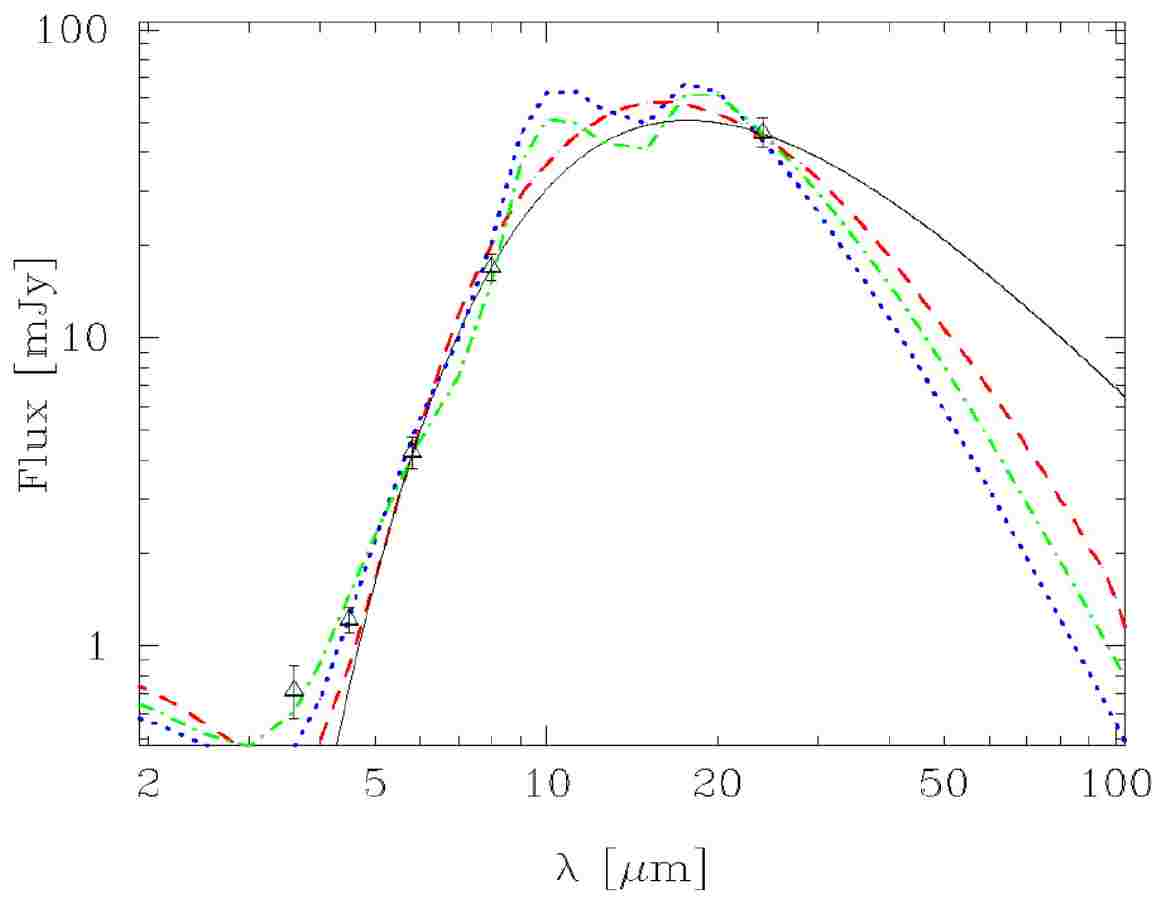
\includegraphics[width=0.5\textwidth,height=!]{./D/barlow_sn2002hh_fig2.jpg}
\end{center}
\vfill The modelling of the radiatively heated dust in SN~2002hh
yields a total dust mass of 0.10--0.15~M$_\odot$, giving a progenitor
mass of $\sim$10--15~M$_\odot$. The parameters of the dust shell are
reminiscent of those around Galactic LBVs: a radius of 0.5--1~pc, dust
masses of 0.1--0.3~M$_\odot$.


\end{frame}
\begin{frame}\frametitle{SN~2002hh.}

\begin{itemize}

\item The IR luminosity of SN~2002hh at day 600 is $\sim
  10^7$L$_\odot$, much higher than that expected for the SN ejecta. 


\item Hence the observed mid-IR emission is due to flash-heated dust,
  a kind of ``thermal echo''. 

\item The thermal echo interpretation, rather than the condensation of
  dust in the SN ejecta, is also supported by the absence of line
  asymmetries in SN~2002hh for the same epoch (Clayton \& Welsh 2004,
  AAS meeting).

\item By comparison, SN~1987A scaled to the distance of SN~2002hh
  would have a factor of 35 less mid-IR flux at the same epoch.


\end{itemize}

\end{frame}
\begin{frame}\frametitle{Dust condensation and emission line asymmetry.}

\begin{itemize}
\item Among the discoveries in SN 1987A, oberved around day 600 but
  largely unexploited, is the asymmetry of optical emission lines
  generated by dust internal to the ejecta (Danziger et al. 1989, IAUC
  4746).  Dust condenses during the cooling related to the violent
  expansion, after day $\sim 300$. Dust absorption extinguishes the
  red-shifted side of the metal-rich ejecta, thereby blue-shifting the
  obserbed profiles. Scattering off dust in an expanding nebula should
  also generate a red tail in the emission line profiles.

%
%\item The modelling of line profile from species of similar excitation
%  but varying wavelength will separate the effects of dust from the
%  kinematics, and yield morphological information.
%
%\item In a first approximation the dust optical properties will be
%  kept fixed as standard ISM.  We will test the data for deviations
%  from the standard extinction law, and consider including the
%  wavelength-dependent cross sections of condensed dust as free
%  parameters.
%
\end{itemize}


\end{frame}



\begin{frame}\frametitle{Dust condensation in Cas A.}



\begin{center}
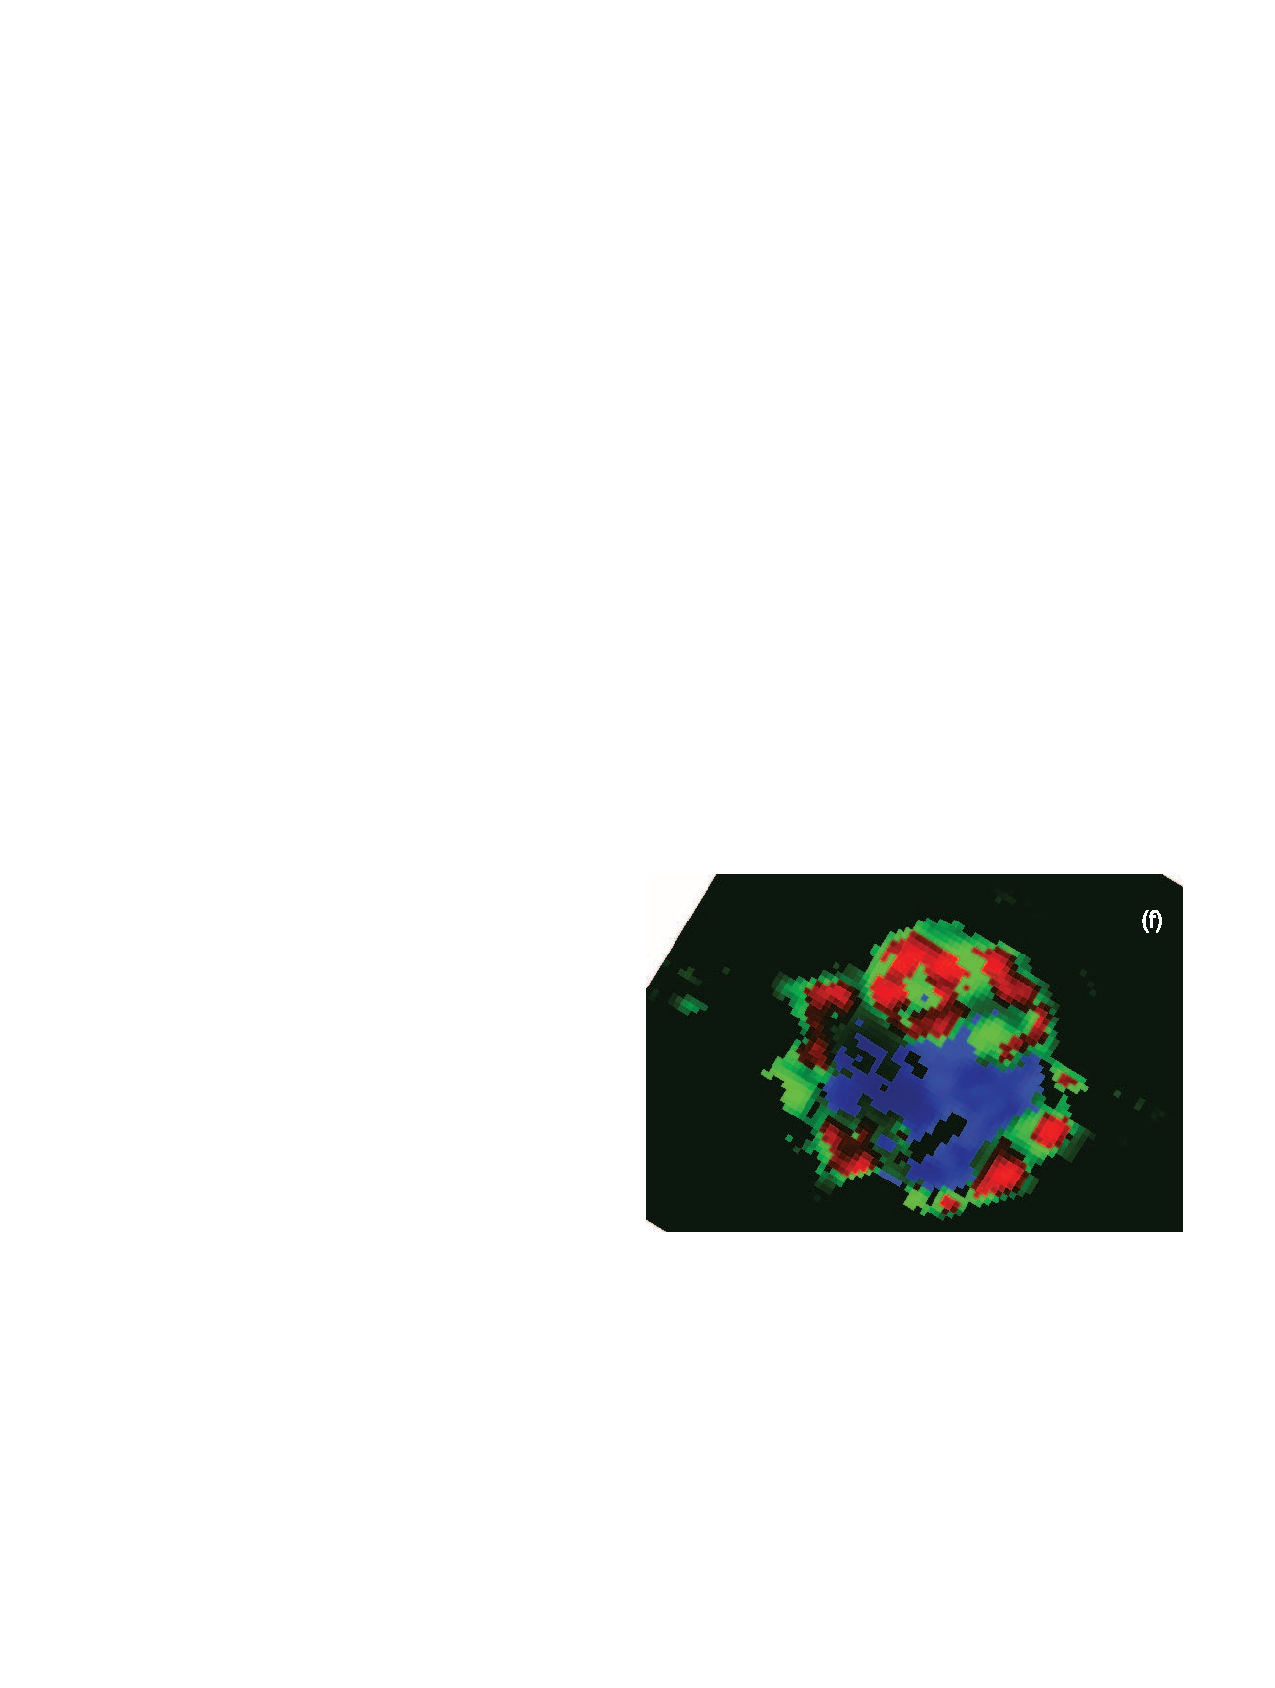
\includegraphics[width=0.5\textwidth,height=!]{./D/rho_etal_fig2.pdf}
\end{center}

Rho et al. 2008. 

\end{frame}




%
%\foilhead{\textcolor{red}{D-\ref{item:dustcycle}} Evolution of dust:
%SNe as dust factories}
%
%Bouchet et al. (2004, ApJ, 611, 394) found and IR point source at the
%location of the envelope ejected by SN1987A, with
%$10^{-3}$~M$_{\odot}$ in dust:
%\vspace{-0.1cm}
%\begin{center}
%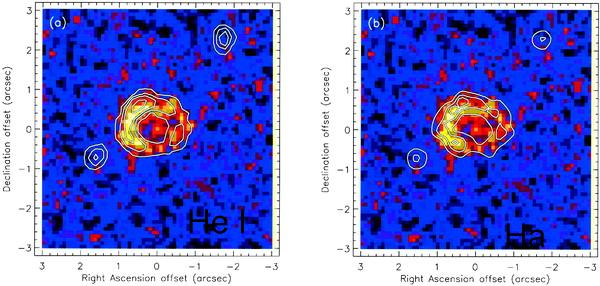
\includegraphics[width=15cm,height=!]{./D/SN1987A_1.jpg}
%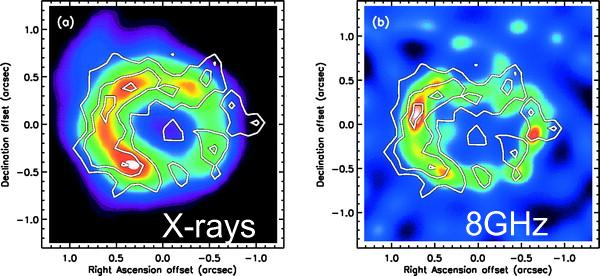
\includegraphics[width=15cm,height=!]{./D/SN1987A_2.jpg}
%\end{center}
%\vfill

\begin{frame}\frametitle{Evolution of dust:
Condensation in hostile environments}

\medskip
\medskip
\medskip
\begin{minipage}[t]{0.55\textwidth}
\begin{center}
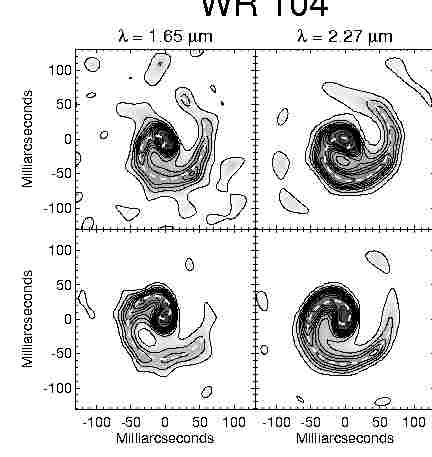
\includegraphics[width=0.99\textwidth,height=!]{./D/WR104.jpg}
\end{center}
\end{minipage}
\hfill
\begin{minipage}[t]{0.44\textwidth}
\begin{center}
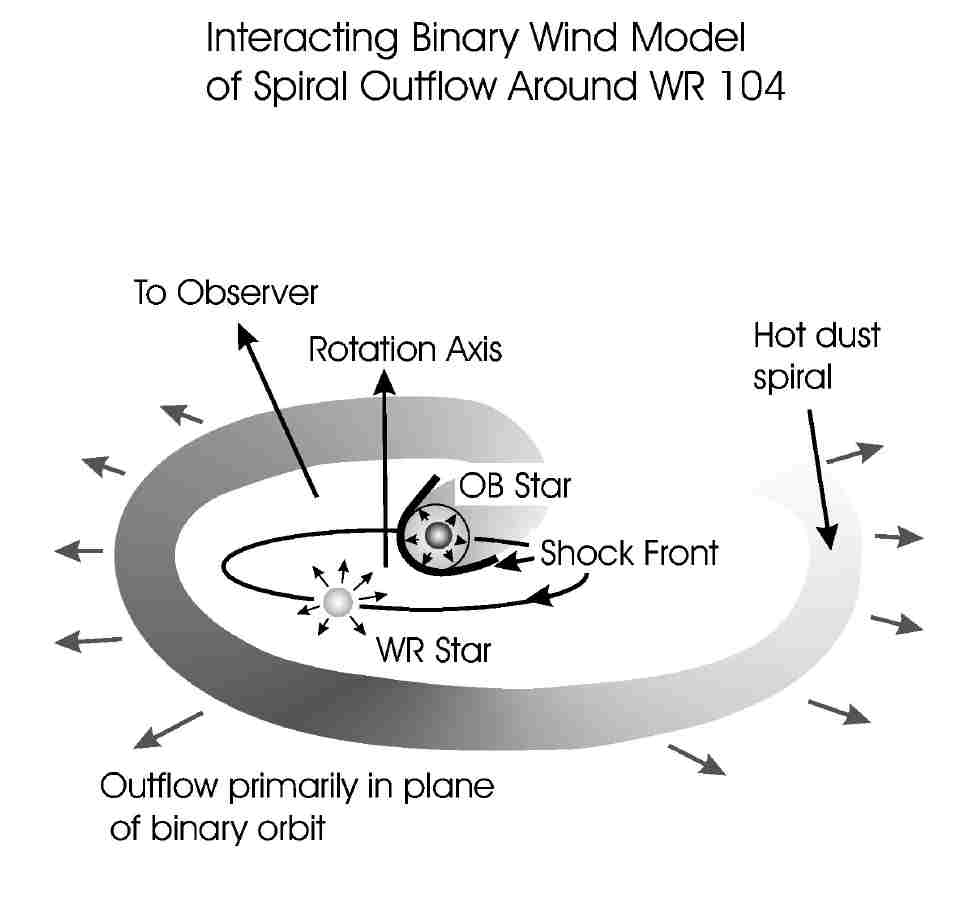
\includegraphics[width=\textwidth,height=!]{./D/WR104_mod.jpg}
\end{center}
\end{minipage}


\end{frame}
\begin{frame}\frametitle{ Evolution of dust:
survival in ionised regions}

\begin{itemize}

\item The refractory elements (with high condensation temperatures)
are systematically underabundant in H\,{\sc ii} regions, even in the
presence of intense X-ray fields (Aller et al. 1981, Pwa et al., 1984,
1986, Oliva et al. 1996, Kingdon \& Ferland 1997, Casassus et
al. 2000).

\item There is an IR excess in the direction of H\,{\sc ii} regions
  (Spitzer 1978). 

\item Ercolano et al. (2003, MNRAS, 344, 1145) show it is necessary to
include the photoelectric effect in order to raise the temperature of
regions with super-solar metallicity (in particular in the models with
dual chemistries required to explain the ORL/CEL discrepancy).

\end{itemize}

\end{frame}
\begin{frame}\frametitle{ Evolution of dust:
destruction of dust and time scales\footnote{Draine, B.T., 2004,
ARA\&A, 41, 241}}

\begin{itemize}

\item Presolar grains in meteorites (e.g. in Murchison) show isotopic
anomalies associated to stardust. But this does not imply that the
bulk of the dust in the {\sc ism} is indeed stardust.  

\item {\sc ism} dust is destroyed in SN shock waves (Tielens et
  al. 1994, ApJ, 431, 321), by sputtering from heavy ions in hot gas,
  by grain-grain collisions leading to grain vaporization and
  fragmentation, and by UV exposure, which depletes the VSGs. 

\item   {\em Models} of the evolution of dust grains for  the various
phases of the {\sc ism} {\em show} that the time scale for the
residence of one atom in a given grain is $\tau_\mathrm{dest} \sim
3\,10^8$~yr. 

\item  The rate of star formation in our Galaxy is
$dM/dt\sim 5~$M${_\odot}$~yr$^{-1}$, and the total mass of the ISM is
$M_\mathrm{ism} \sim 5~10^{9}$M${_\odot}$. The time scale for the
residence of refractory elements in the ISM is thus $\tau_\mathrm{ism}
\approx M_\mathrm{ism}/dMdt \approx 10^9$.

\end{itemize}

\end{frame}
\begin{frame}\frametitle{ Evolution of dust:
destruction of dust and time scales}


\begin{itemize} 

\item Therefore the fraction of $\tau_{\sc ism}$ that a given element
  spends inside a grain is $\tau_\mathrm{dest} / \tau_\mathrm{dest} +
  \tau_\mathrm{ism} = 0.2$ (why not $\tau_\mathrm{dest} /
  \tau_\mathrm{ism}$ ?). $\rightarrow$ if no dust is produced in the
  {\sc ism}, then 20\% of the refractory elements should be locked in dust.


\item But the prediction that  20\% of the refractory elements are in
dust does not match observations, which give up to 90\% for Si
$\rightarrow$ dust is produced in the {\sc ism}

\item The mass of the Milky Way    {\sc ism}  is uncertain to  
1 order of magnitude, and so is the rate of star
formation, and therefore the fraction of Si in grains.



\end{itemize}

\end{frame}
